\chapter{Critical Care}

\begin{figure}
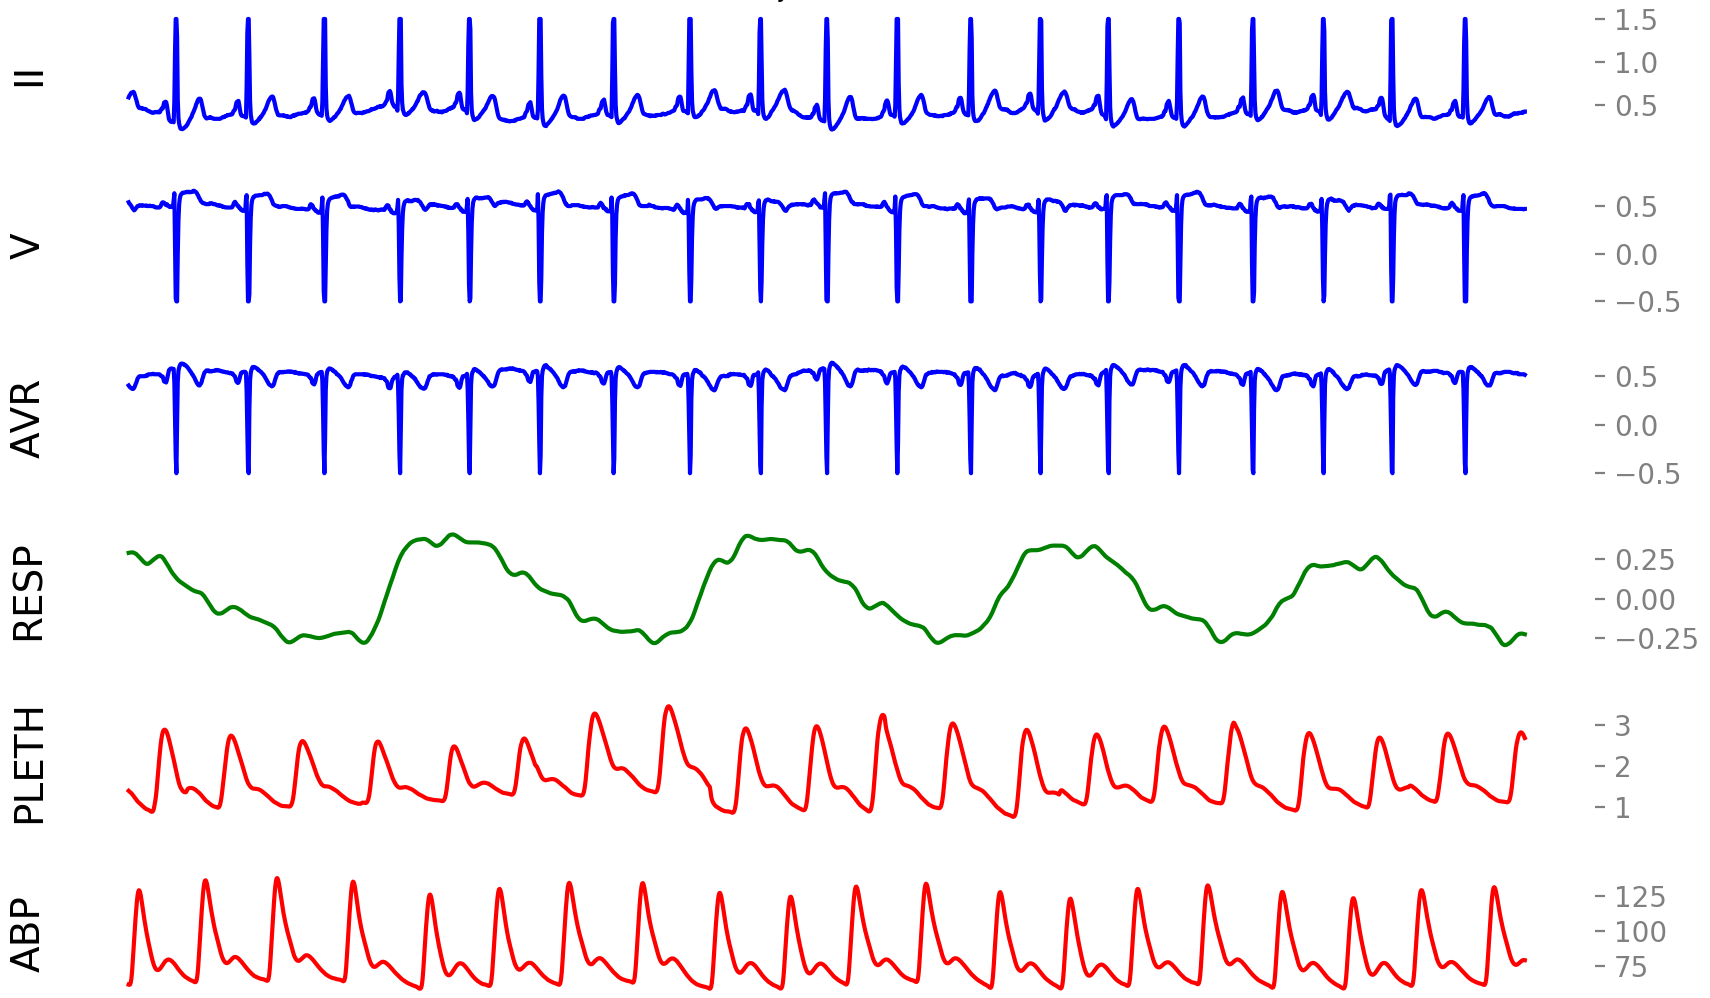
\includegraphics[width=\textwidth]{icu_example_waveforms}
\caption{Example waveforms}
\vspace{12px}
Insert caption here
\label{fig:icu_example_waveforms}
\end{figure}

\begin{figure}
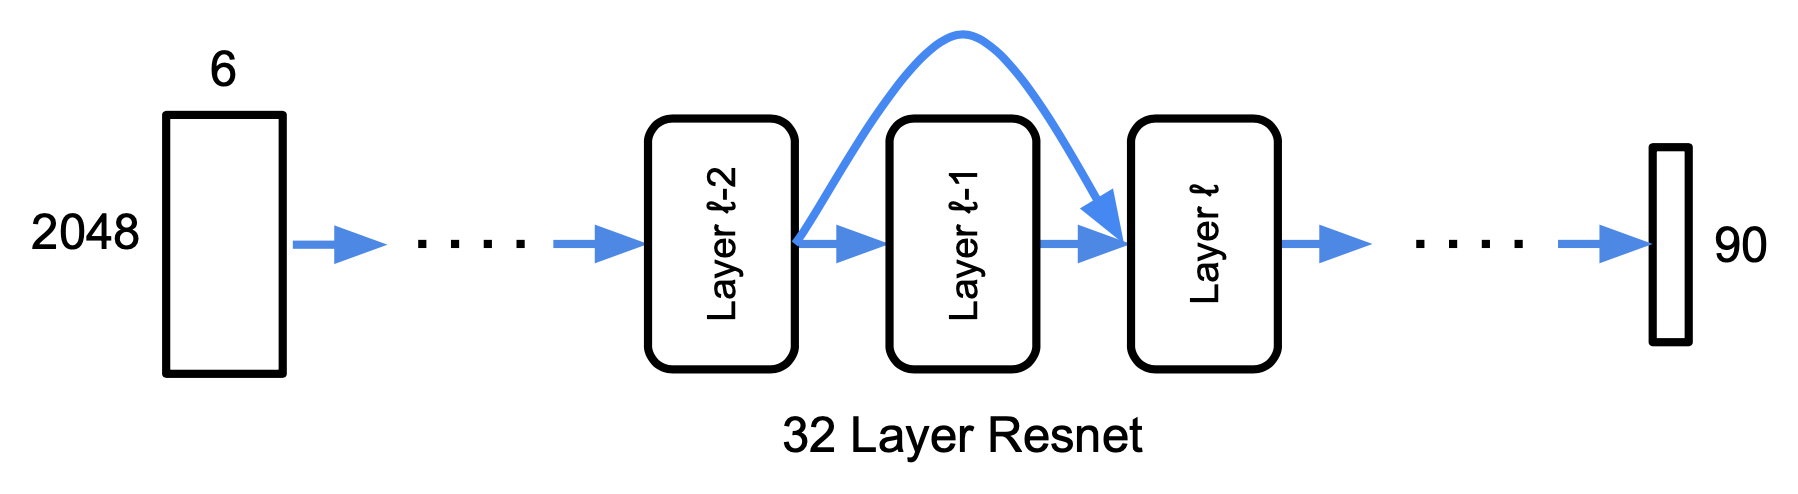
\includegraphics[width=\textwidth]{icu_model_arch}
\caption{Model architecture}
\vspace{12px}
Insert caption here
\label{fig:icu_model_arch}
\end{figure}

\begin{figure}
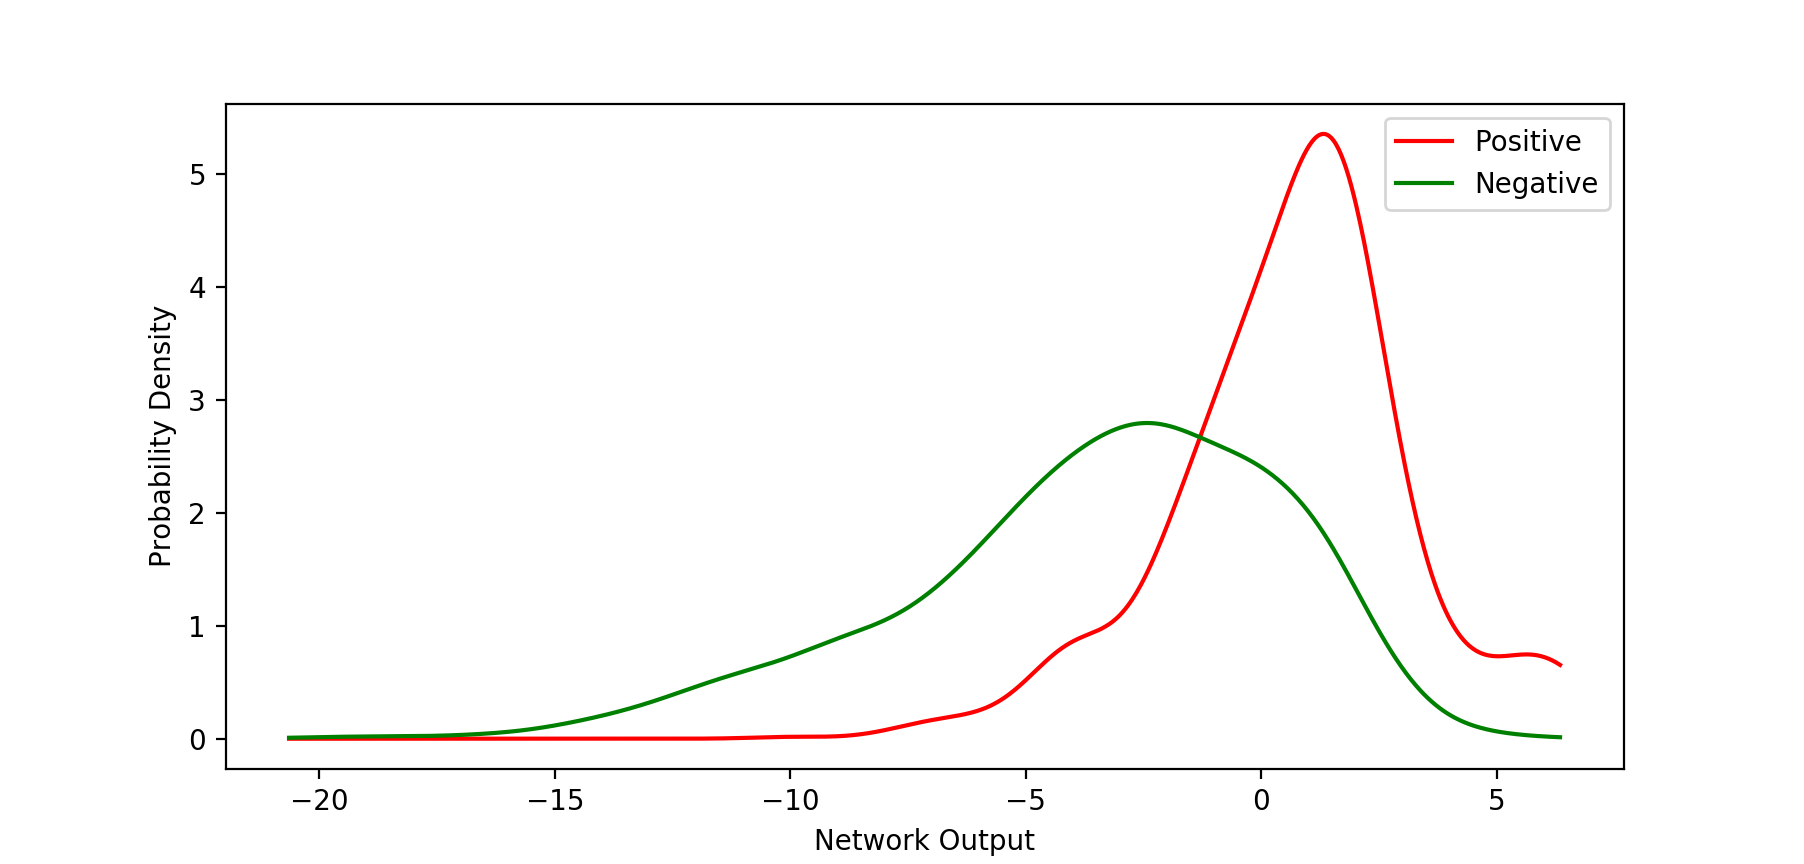
\includegraphics[width=\textwidth]{icu_cardio_prob}
\caption{Cardiogenic Shock Separation}
\vspace{12px}
Insert caption here
\label{fig:icu_cardio_prob}
\end{figure}

\begin{figure}
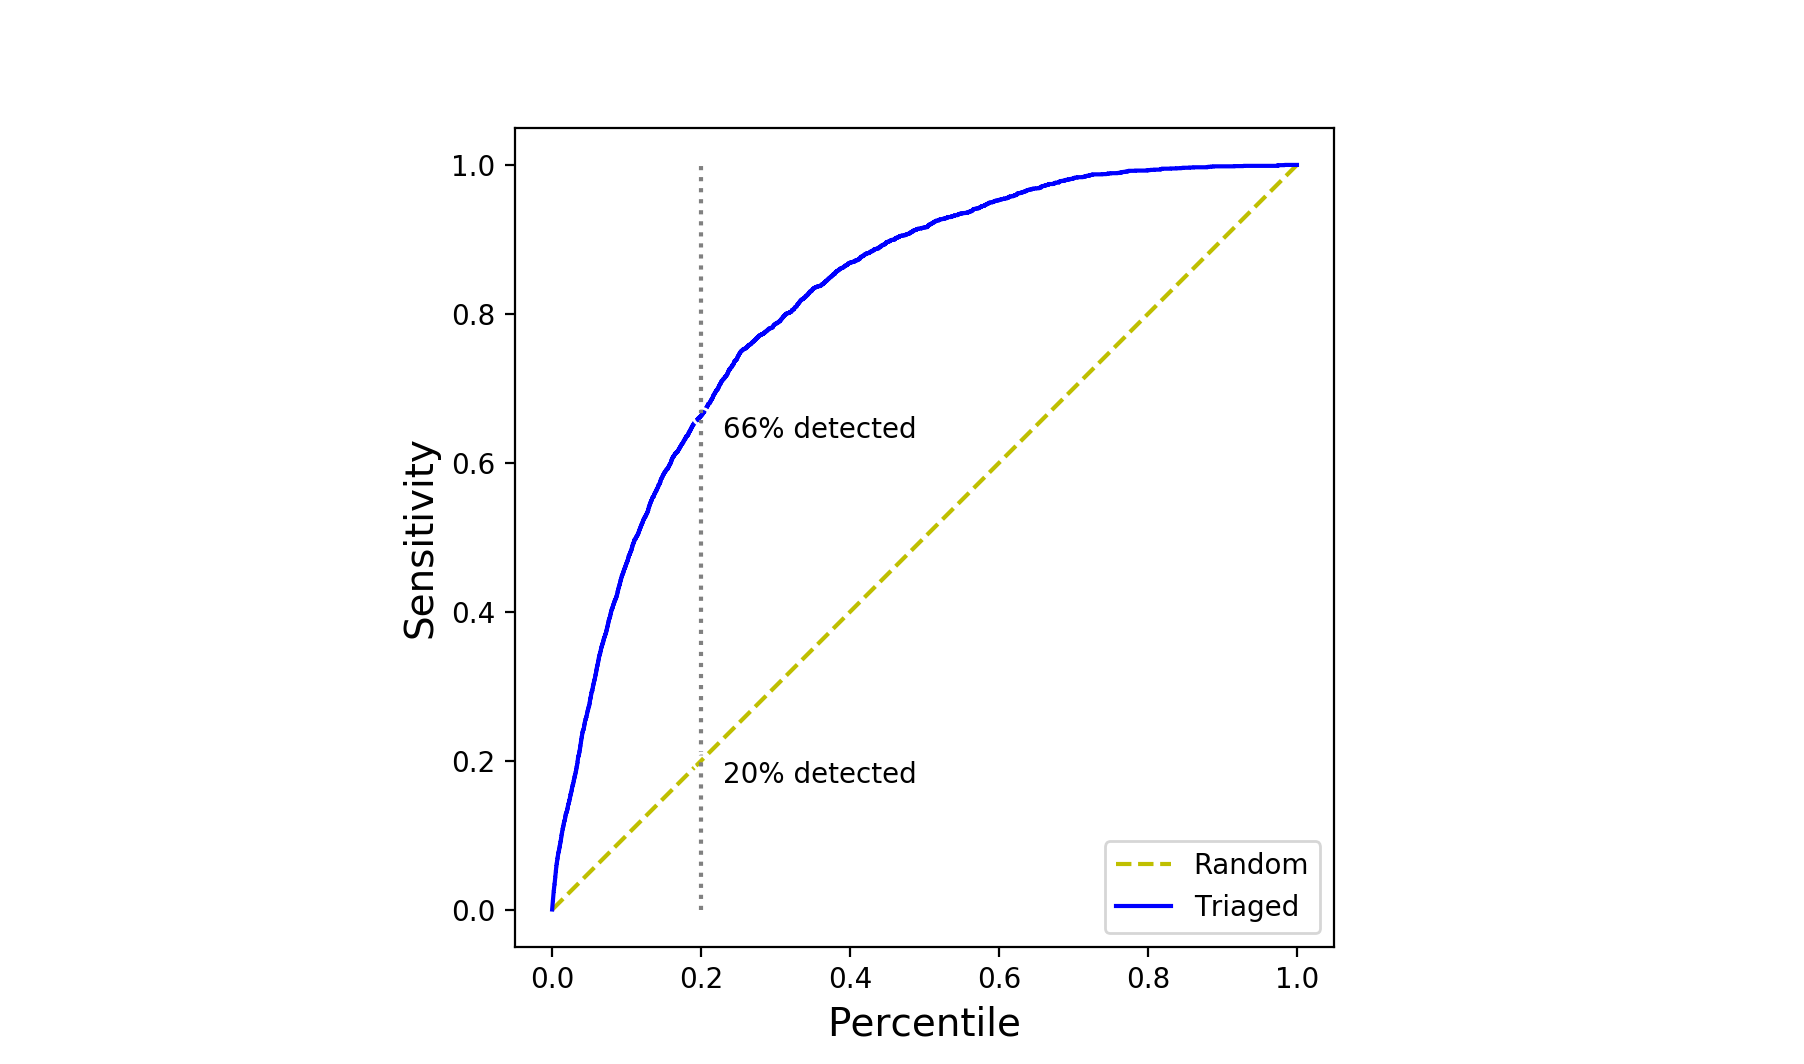
\includegraphics[width=\textwidth]{icu_cardio_sens}
\caption{Cardiogenic Shock Effective Sensitivity}
\vspace{12px}
Insert caption here
\label{fig:icu_cardio_sens}
\end{figure}

\begin{figure}
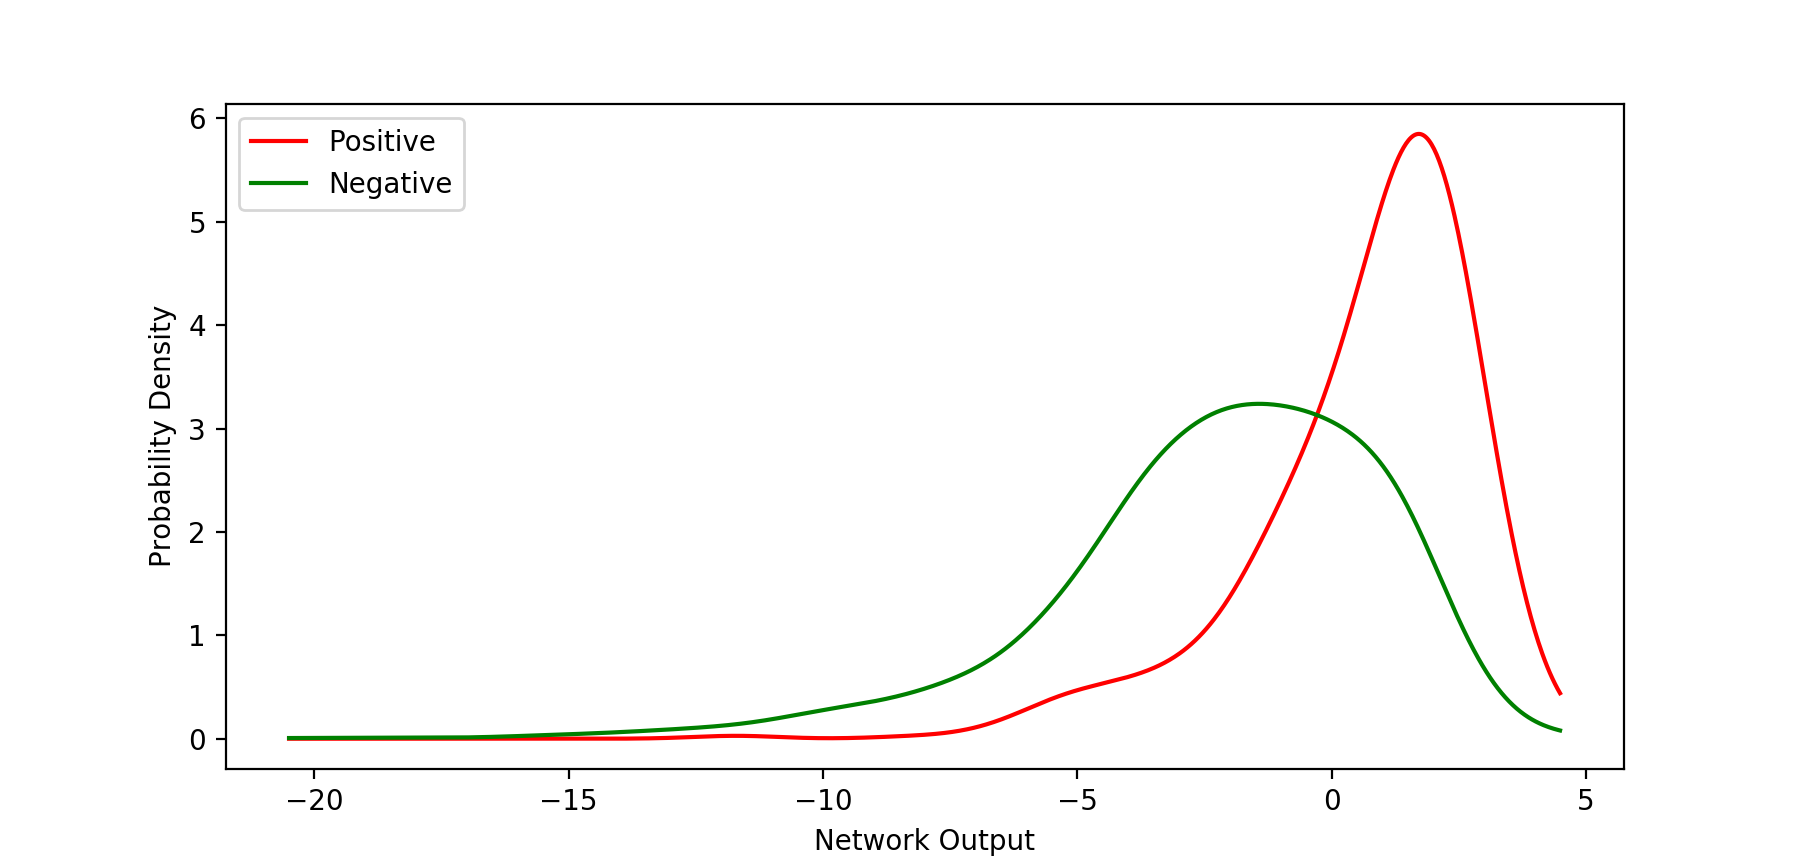
\includegraphics[width=\textwidth]{icu_systolic_prob}
\caption{Systolic Heart Failure Separation}
\vspace{12px}
Insert caption here
\label{fig:icu_systolic_prob}
\end{figure}

\begin{figure}
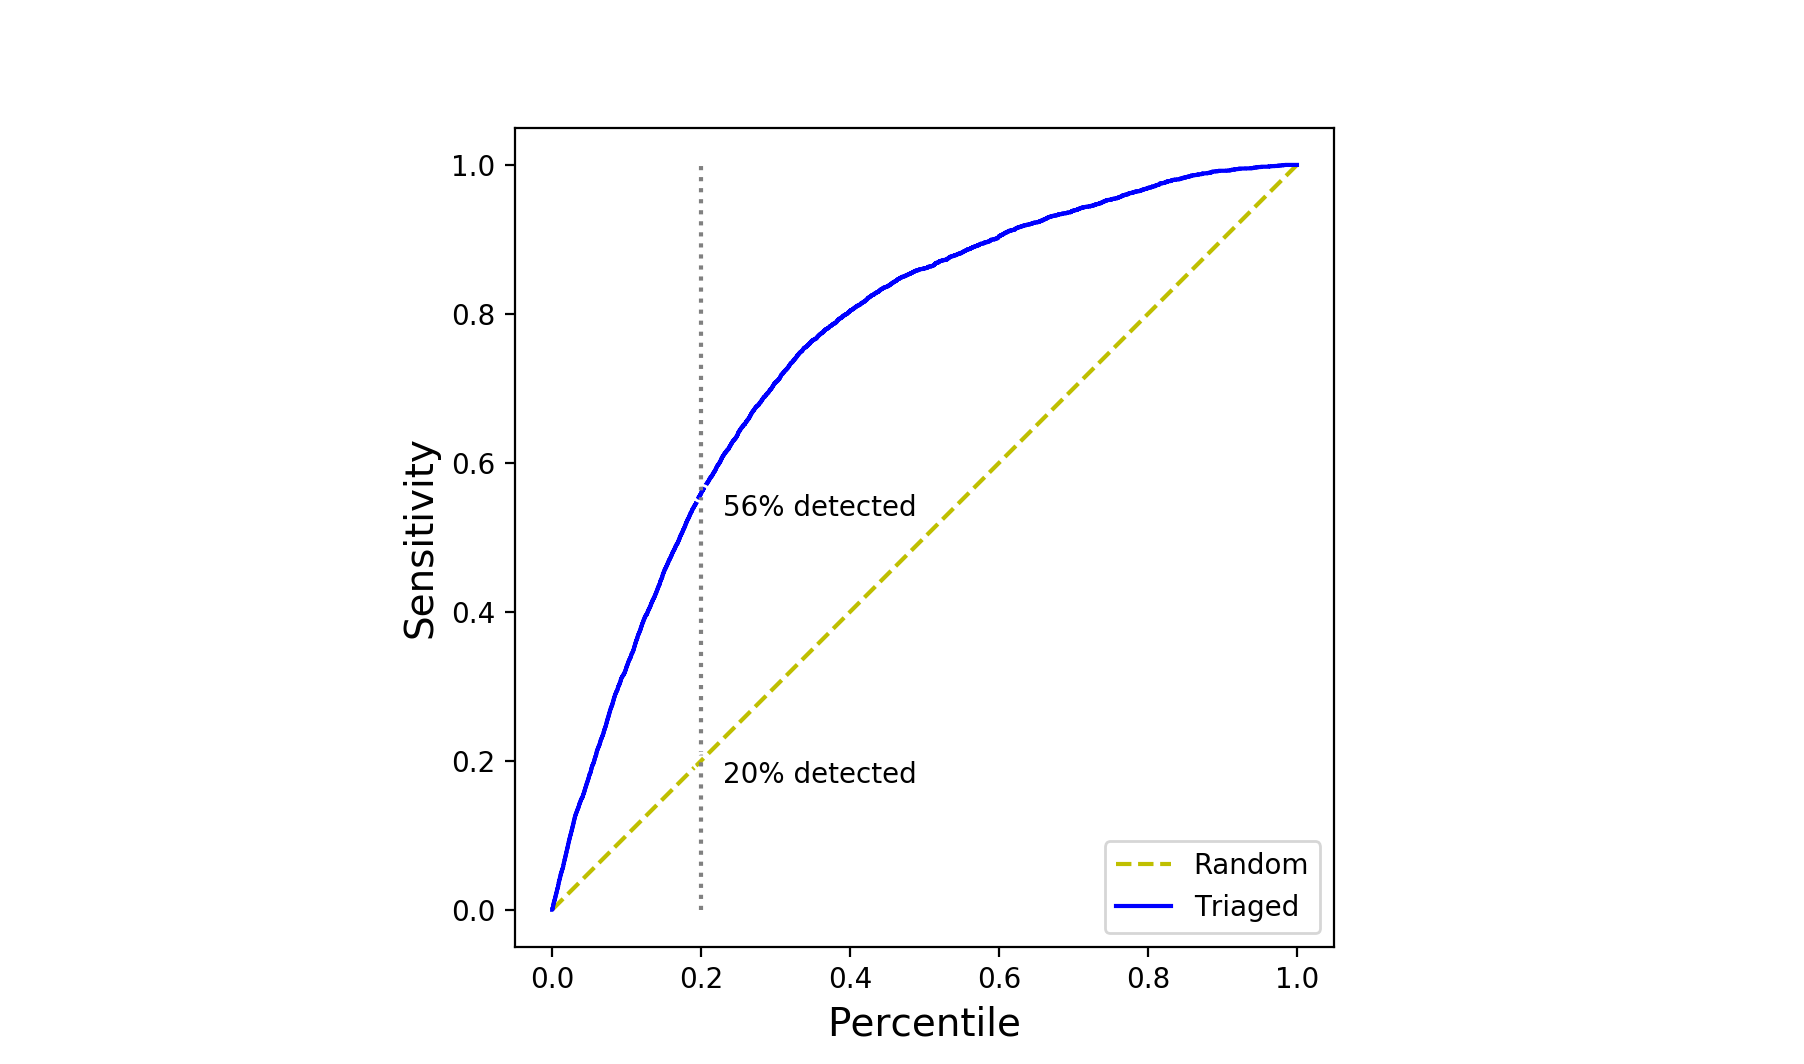
\includegraphics[width=\textwidth]{icu_systolic_sens}
\caption{Systolic Heart Failure Effective Sensitivity}
\vspace{12px}
Insert caption here
\label{fig:icu_systolic_sens}
\end{figure}

\begin{figure}
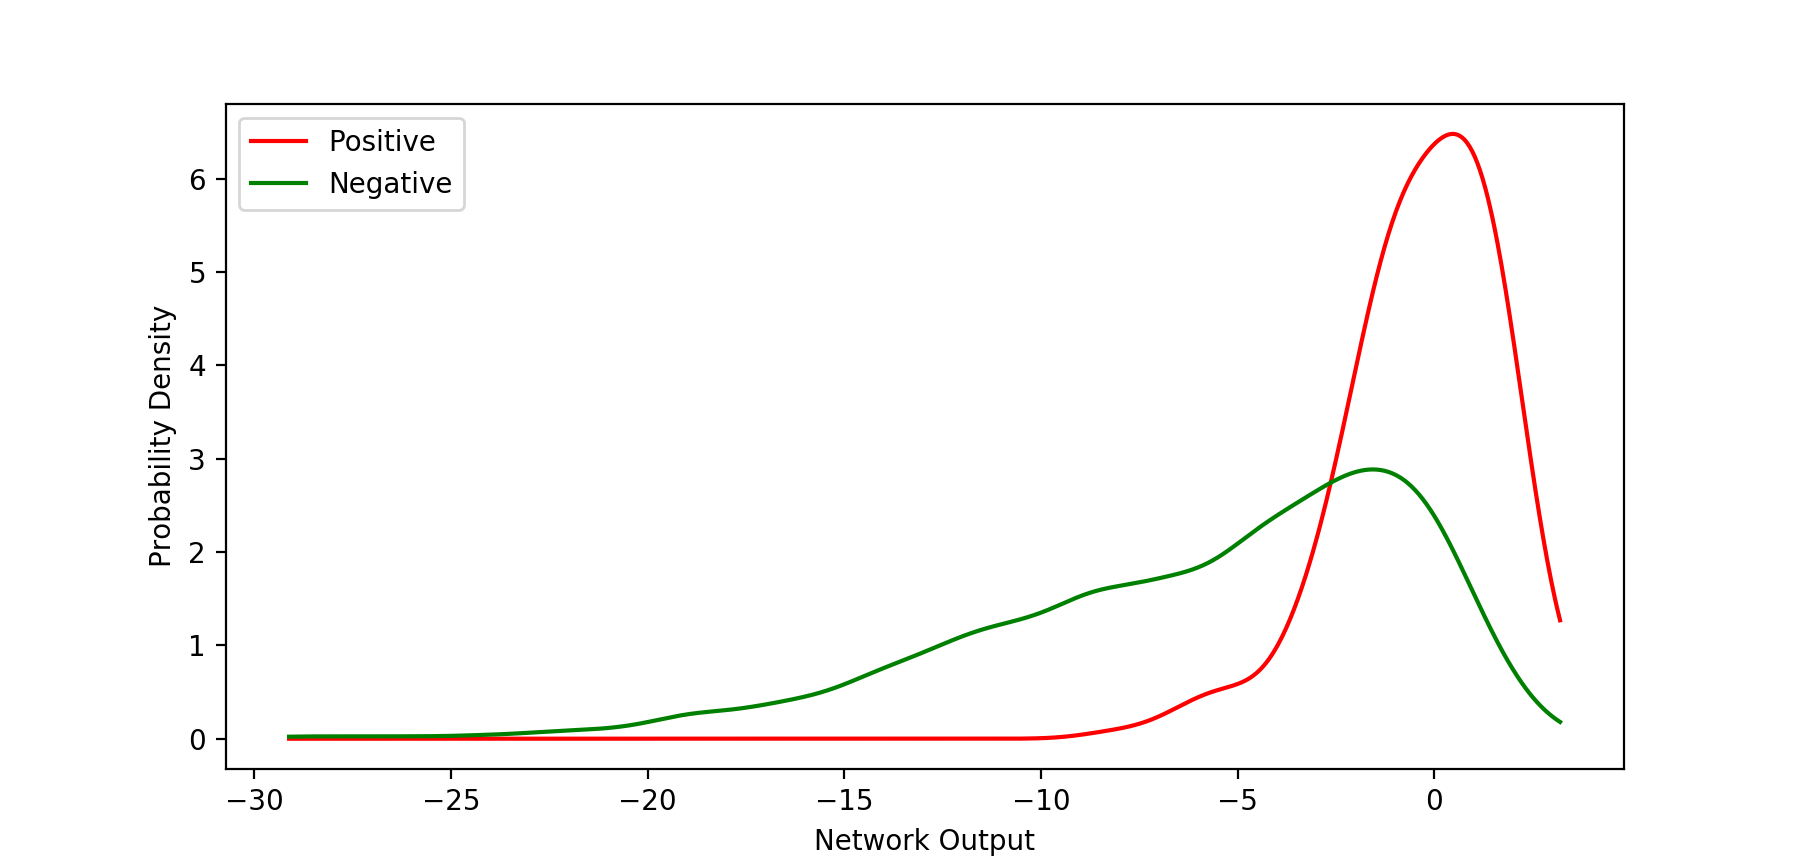
\includegraphics[width=\textwidth]{icu_cerebral_prob}
\caption{Cerebral Aneurysm Separation}
\vspace{12px}
Insert caption here
\label{fig:icu_cerebral_prob}
\end{figure}

\begin{figure}
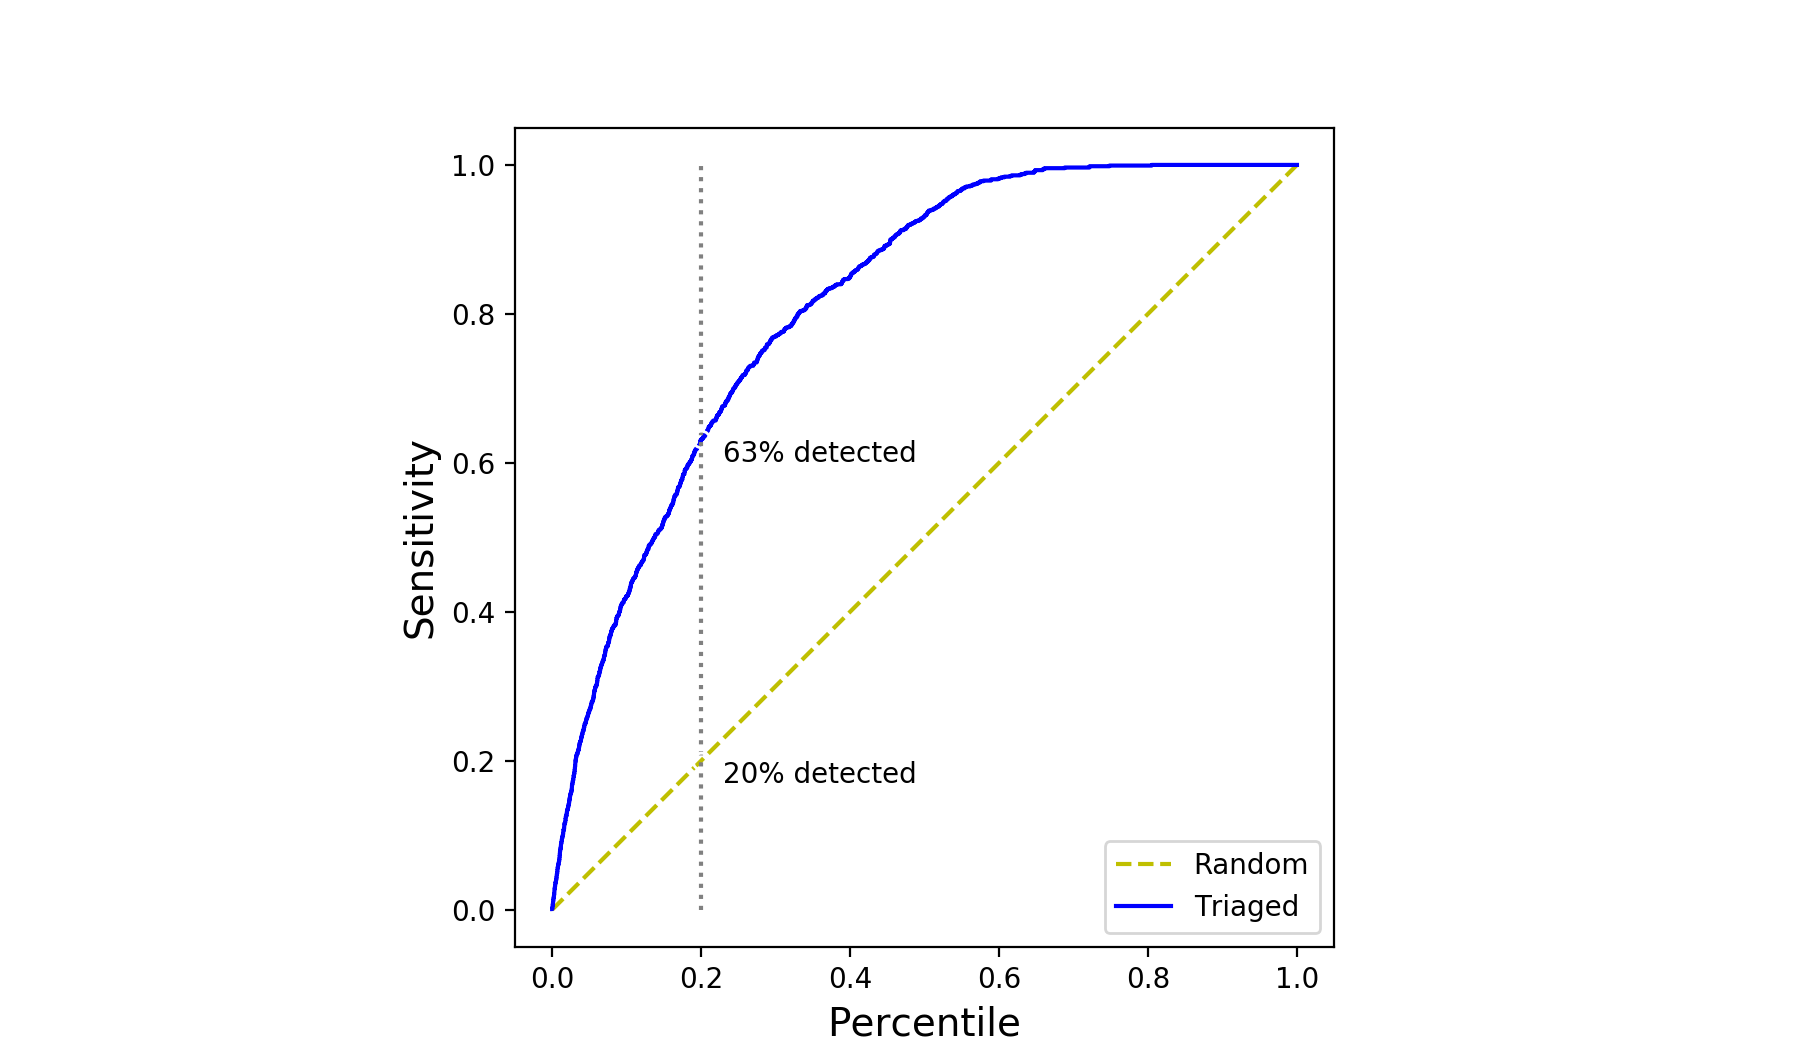
\includegraphics[width=\textwidth]{icu_cerebral_sens}
\caption{Cerebral Aneurysm Effective Sensitivity}
\vspace{12px}
Insert caption here
\label{fig:icu_cerebral_sens}
\end{figure}

\begin{figure}
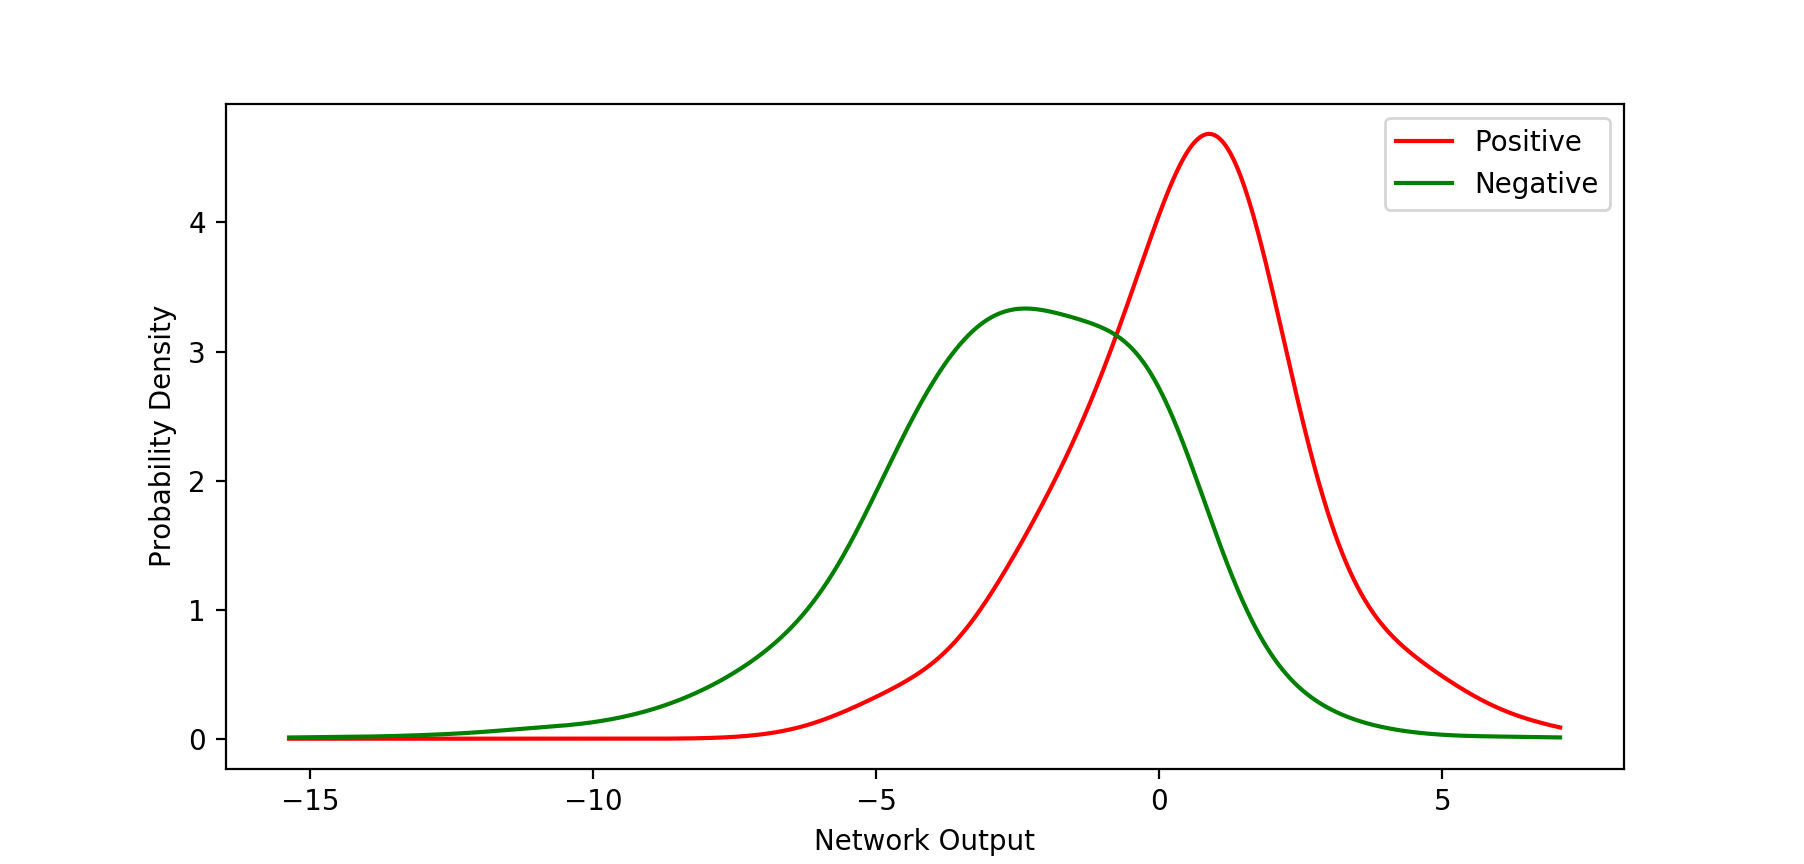
\includegraphics[width=\textwidth]{icu_myocard_prob}
\caption{Myocardial Infarction Separation}
\vspace{12px}
Insert caption here
\label{fig:icu_myocard_prob}
\end{figure}

\begin{figure}
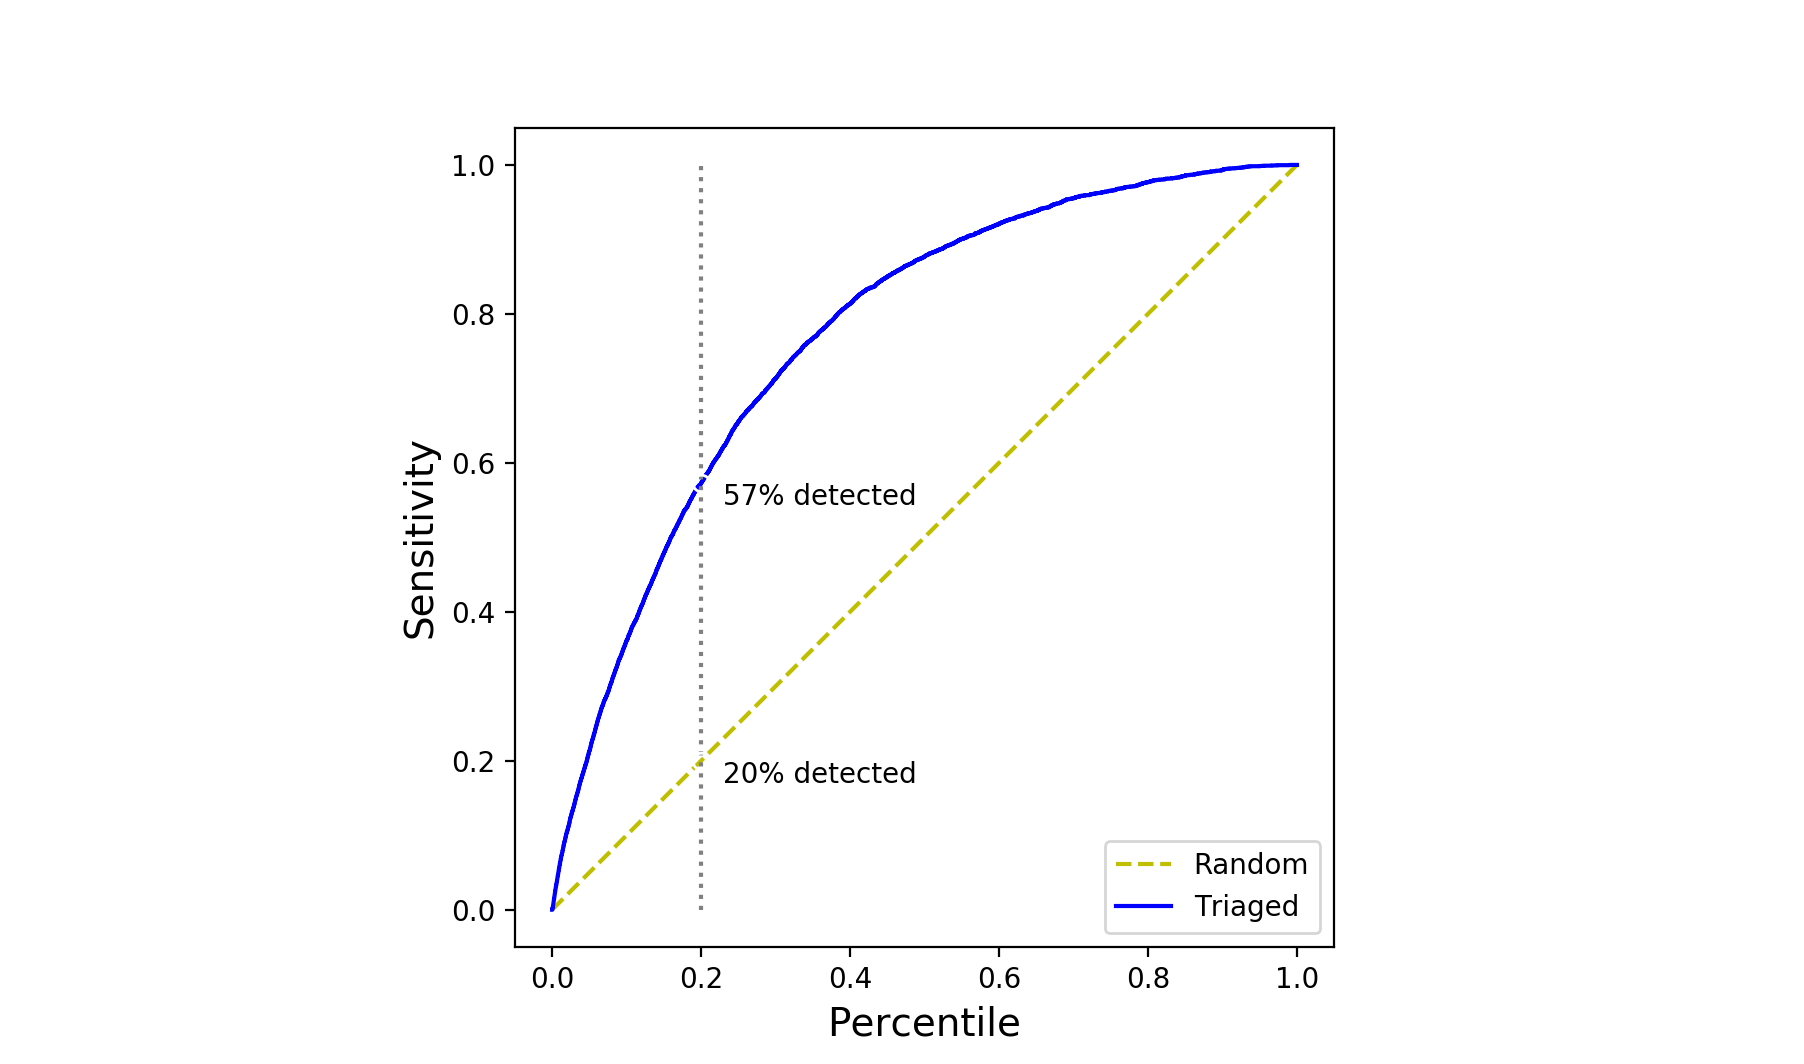
\includegraphics[width=\textwidth]{icu_myocard_sens}
\caption{Myocardial Infarction Effective Sensitivity}
\vspace{12px}
Insert caption here
\label{fig:icu_myocard_sens}
\end{figure}

\begin{figure}
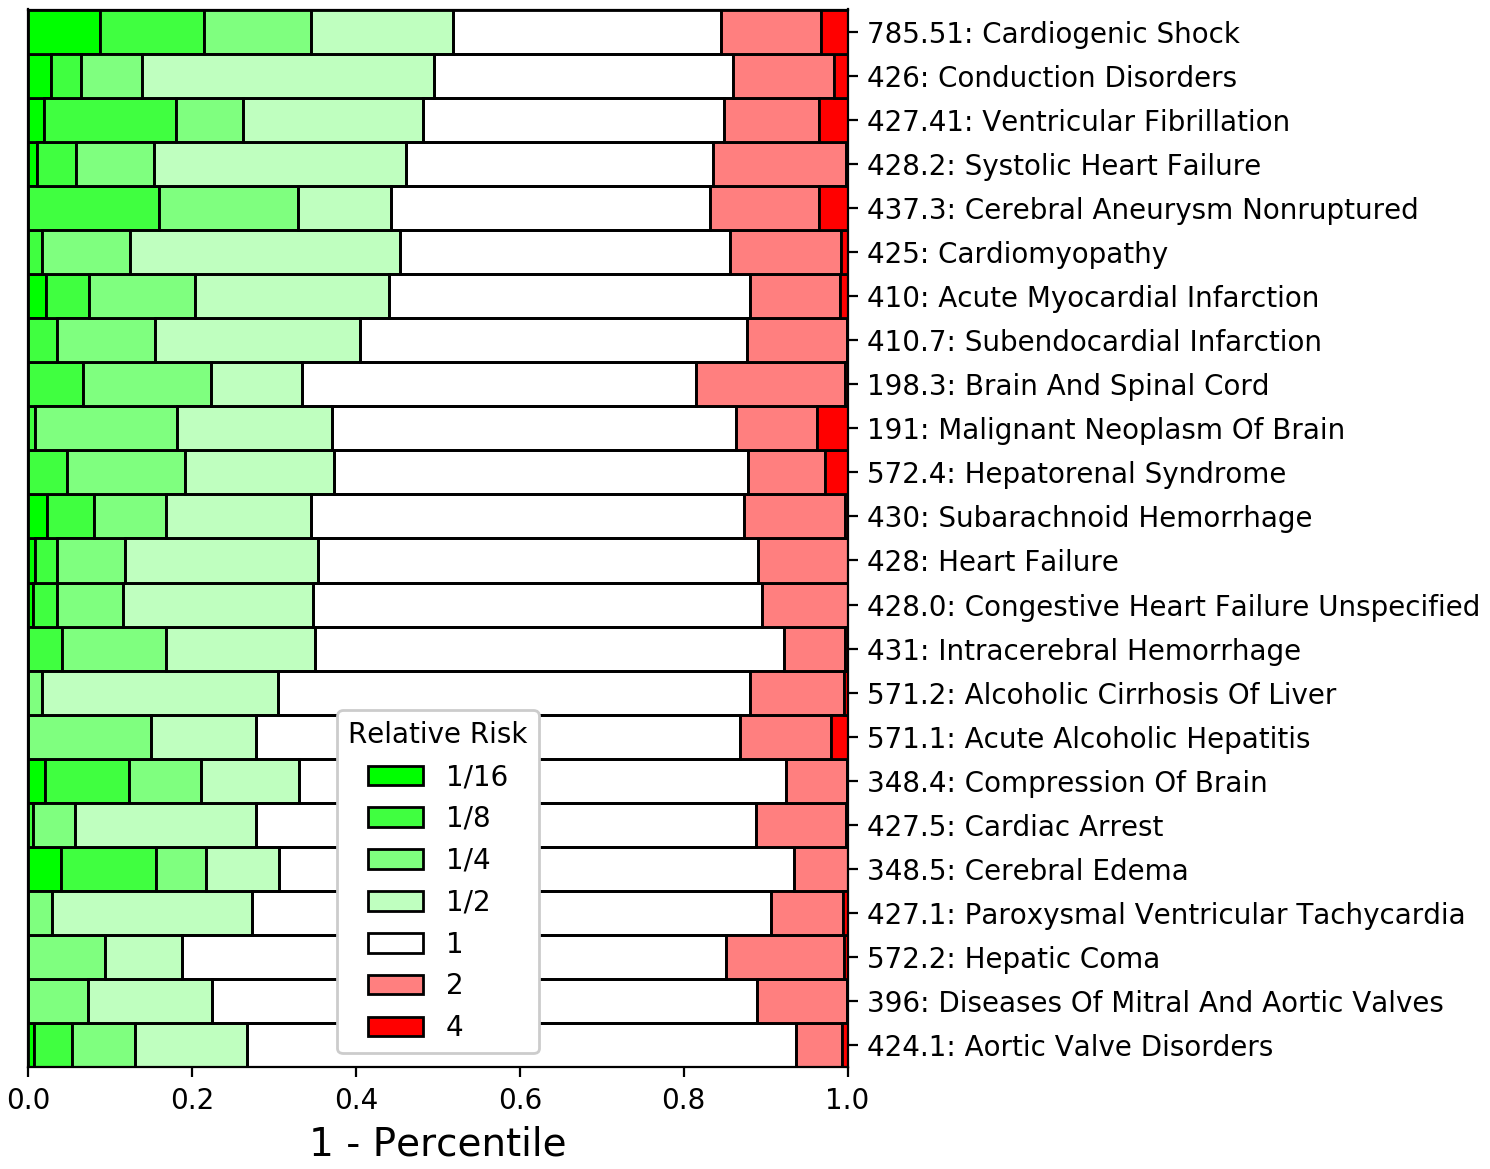
\includegraphics[width=\textwidth]{icu_relative_risk}
\caption{Relative risk}
\vspace{12px}
Insert caption here
\label{fig:icu_relative_risk}
\end{figure}

\begin{figure}
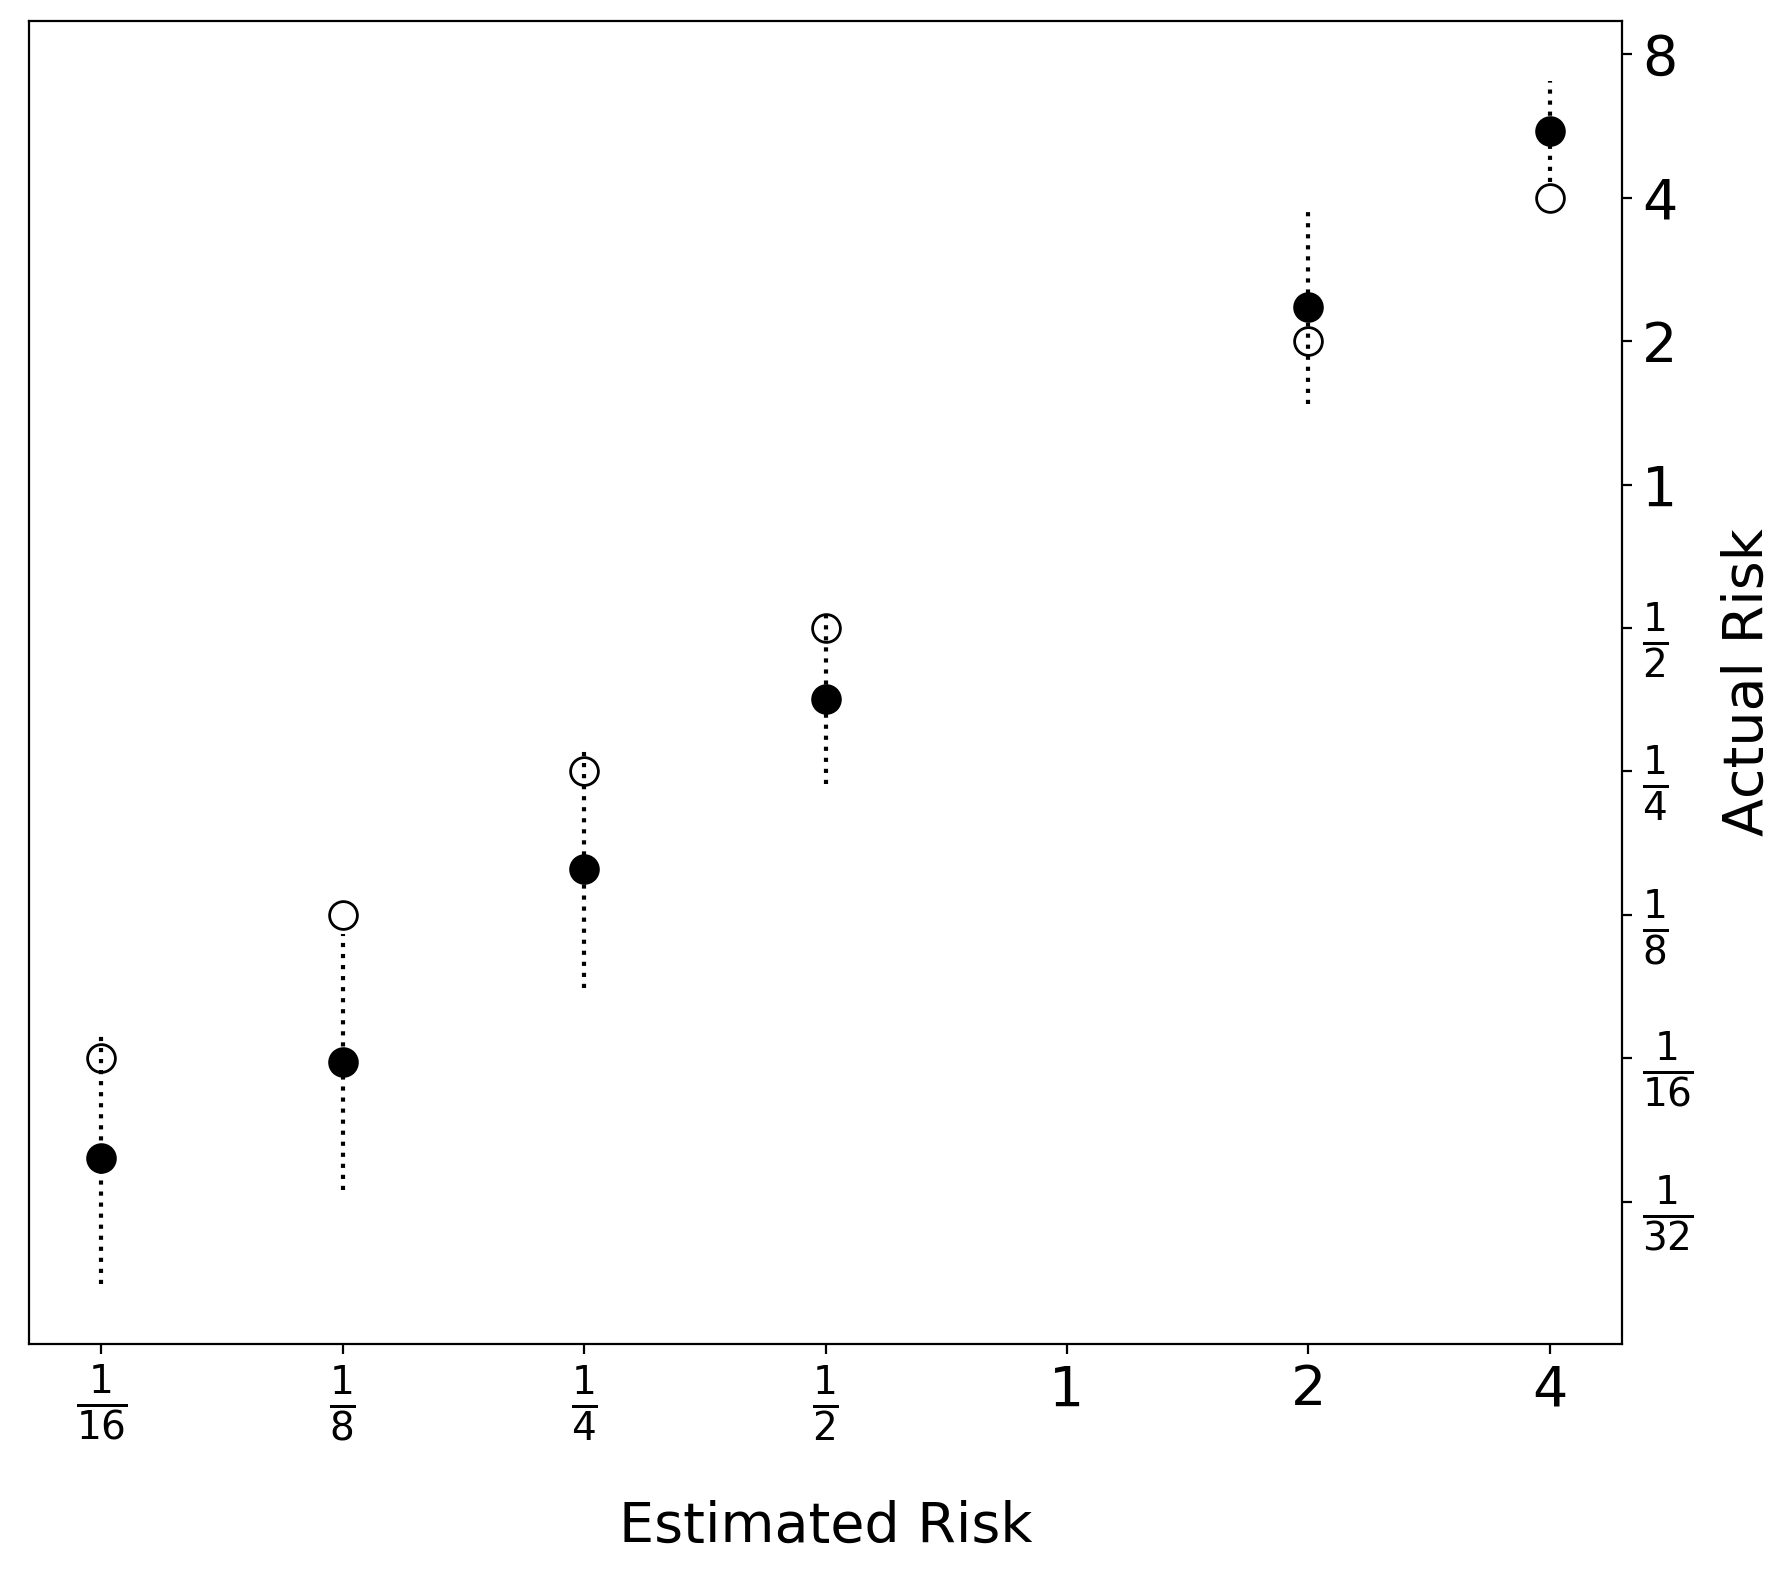
\includegraphics[width=\textwidth]{icu_actual_risk}
\caption{Actual risk}
\vspace{12px}
Insert caption here
\label{fig:icu_actual_risk}
\end{figure}

\begin{figure}
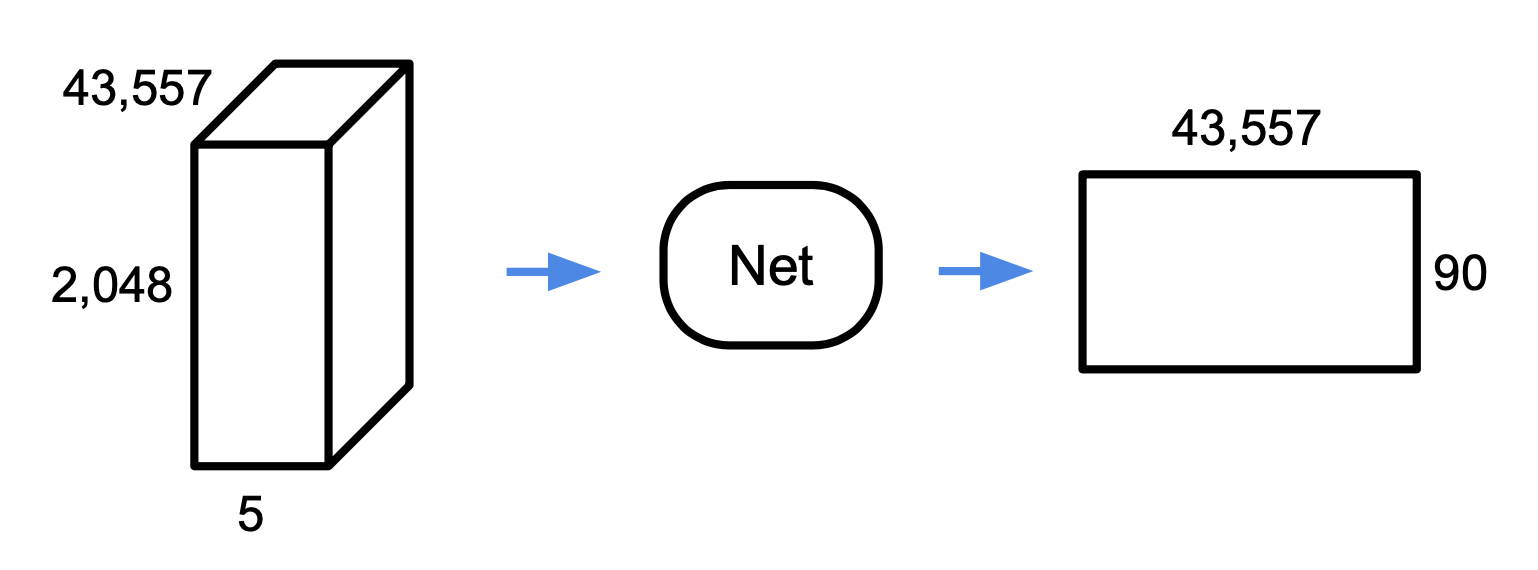
\includegraphics[width=\textwidth]{icu_sem_inf}
\caption{Semantic Inference}
\vspace{12px}
Insert caption here
\label{fig:icu_sem_inf}
\end{figure}

\begin{figure}
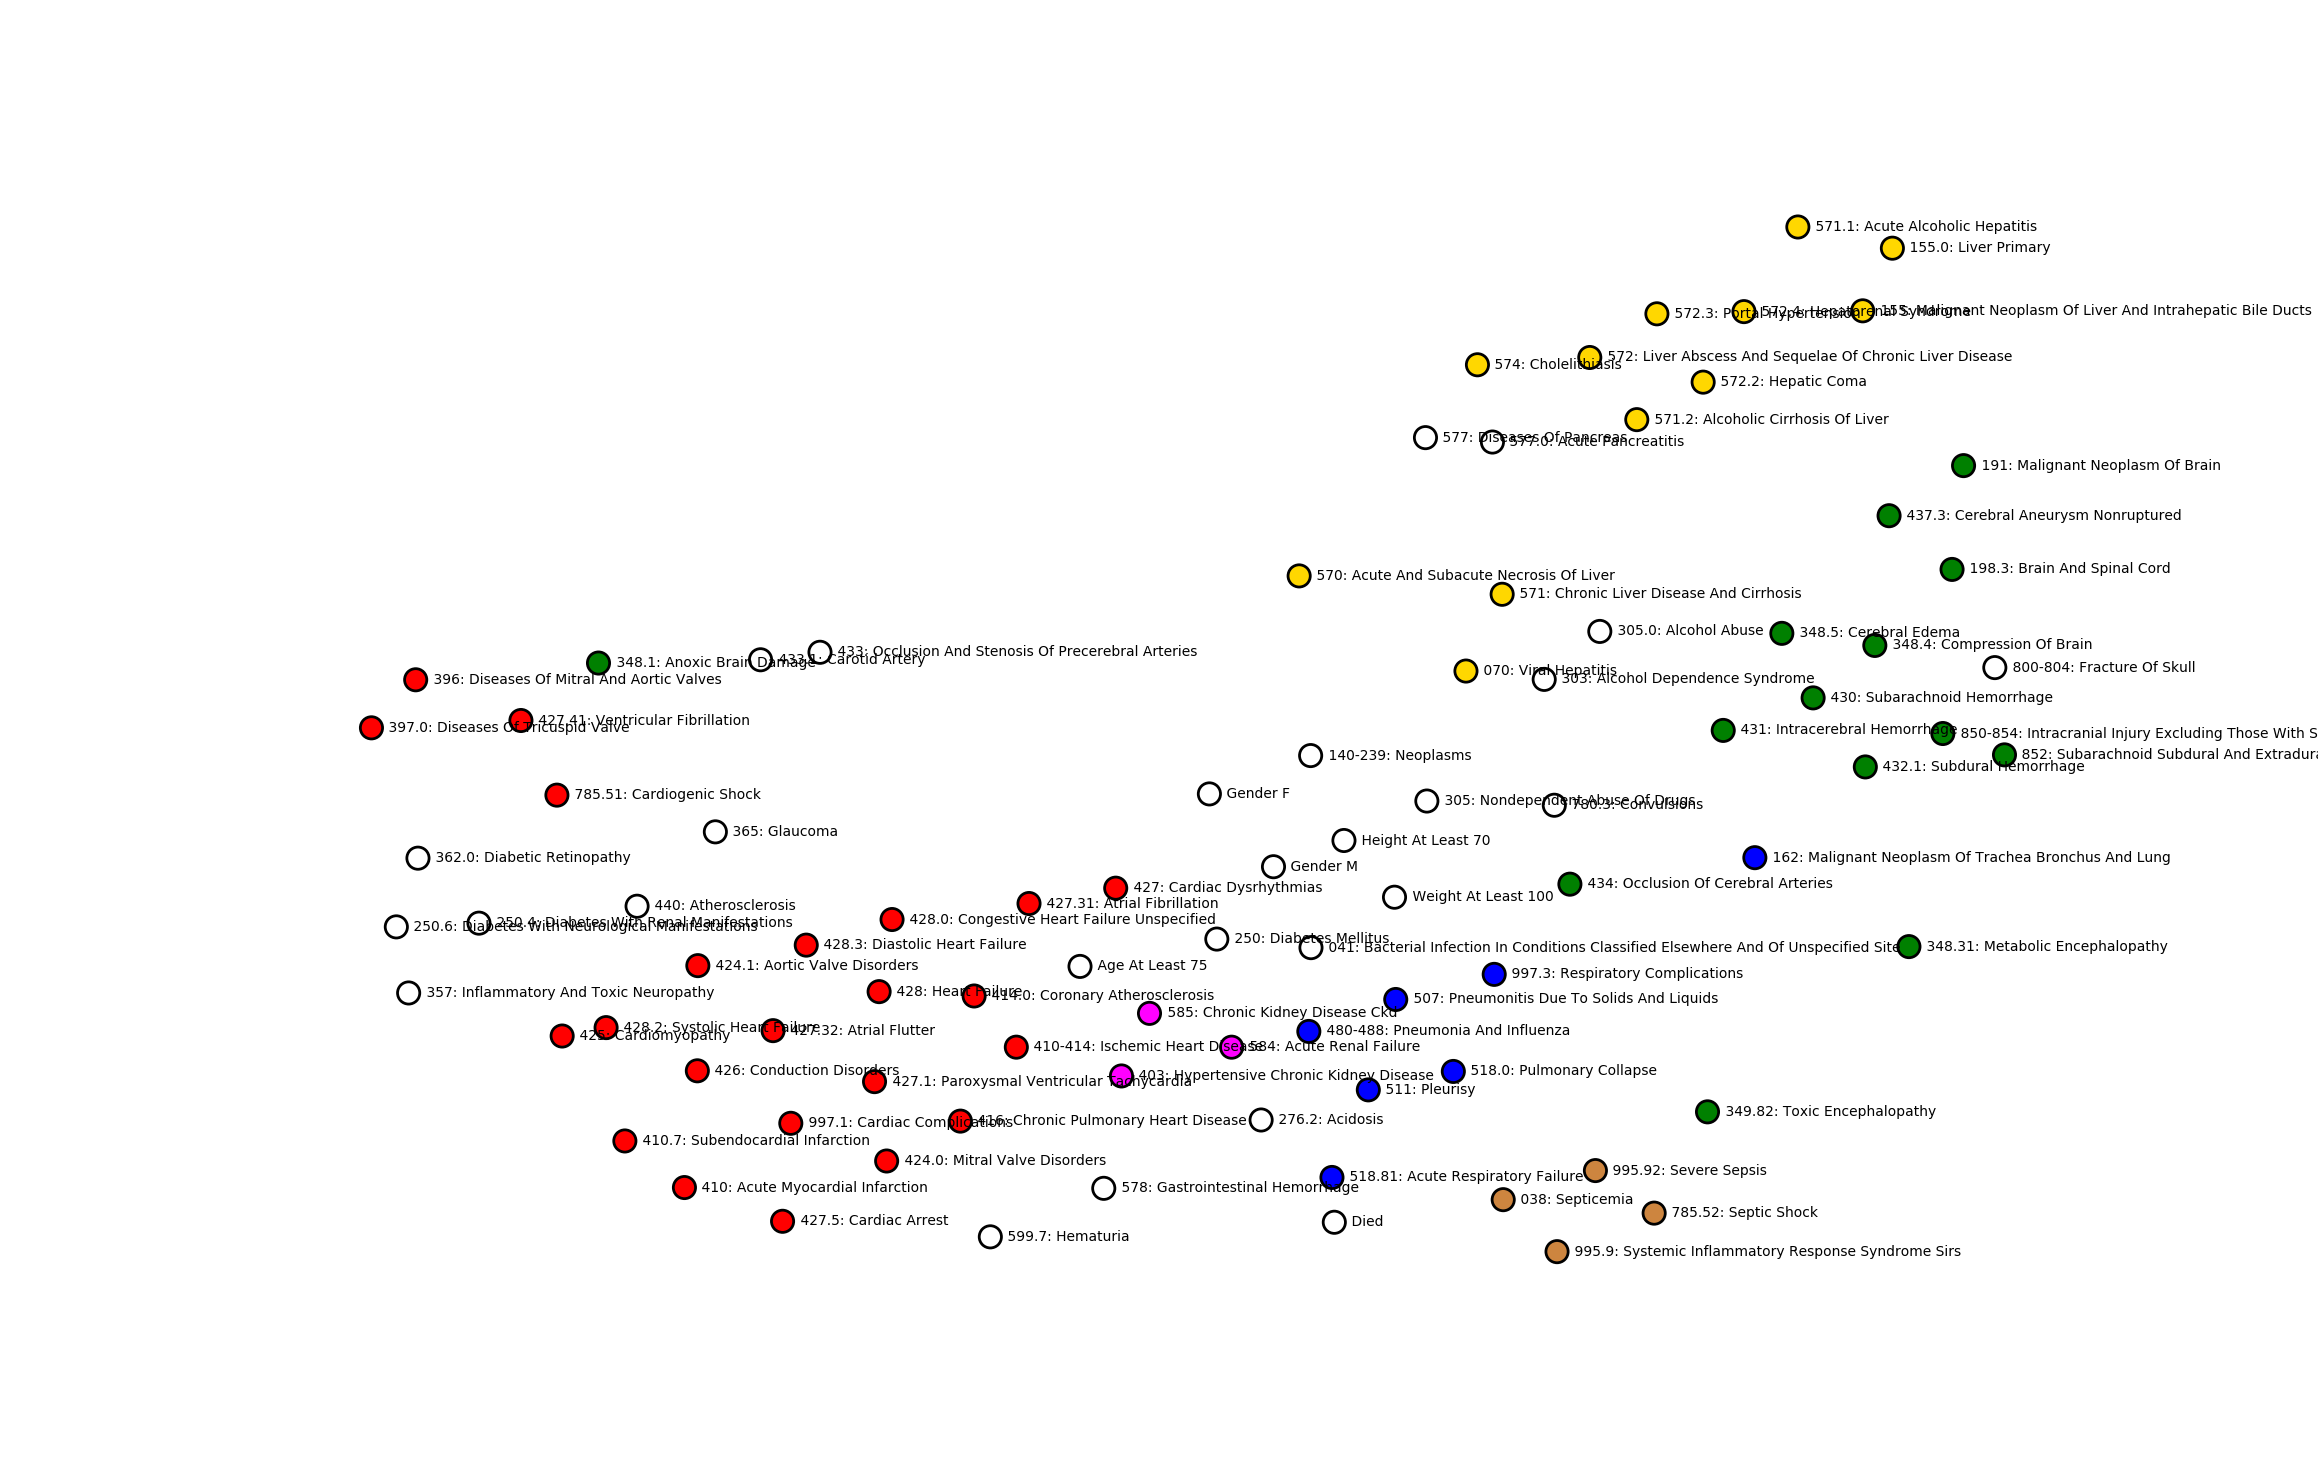
\includegraphics[width=\textwidth]{icu_map}
\caption{Semantic Inference Embedding}
\vspace{12px}
Insert caption here
\label{fig:icu_map}
\end{figure}

\begin{figure}
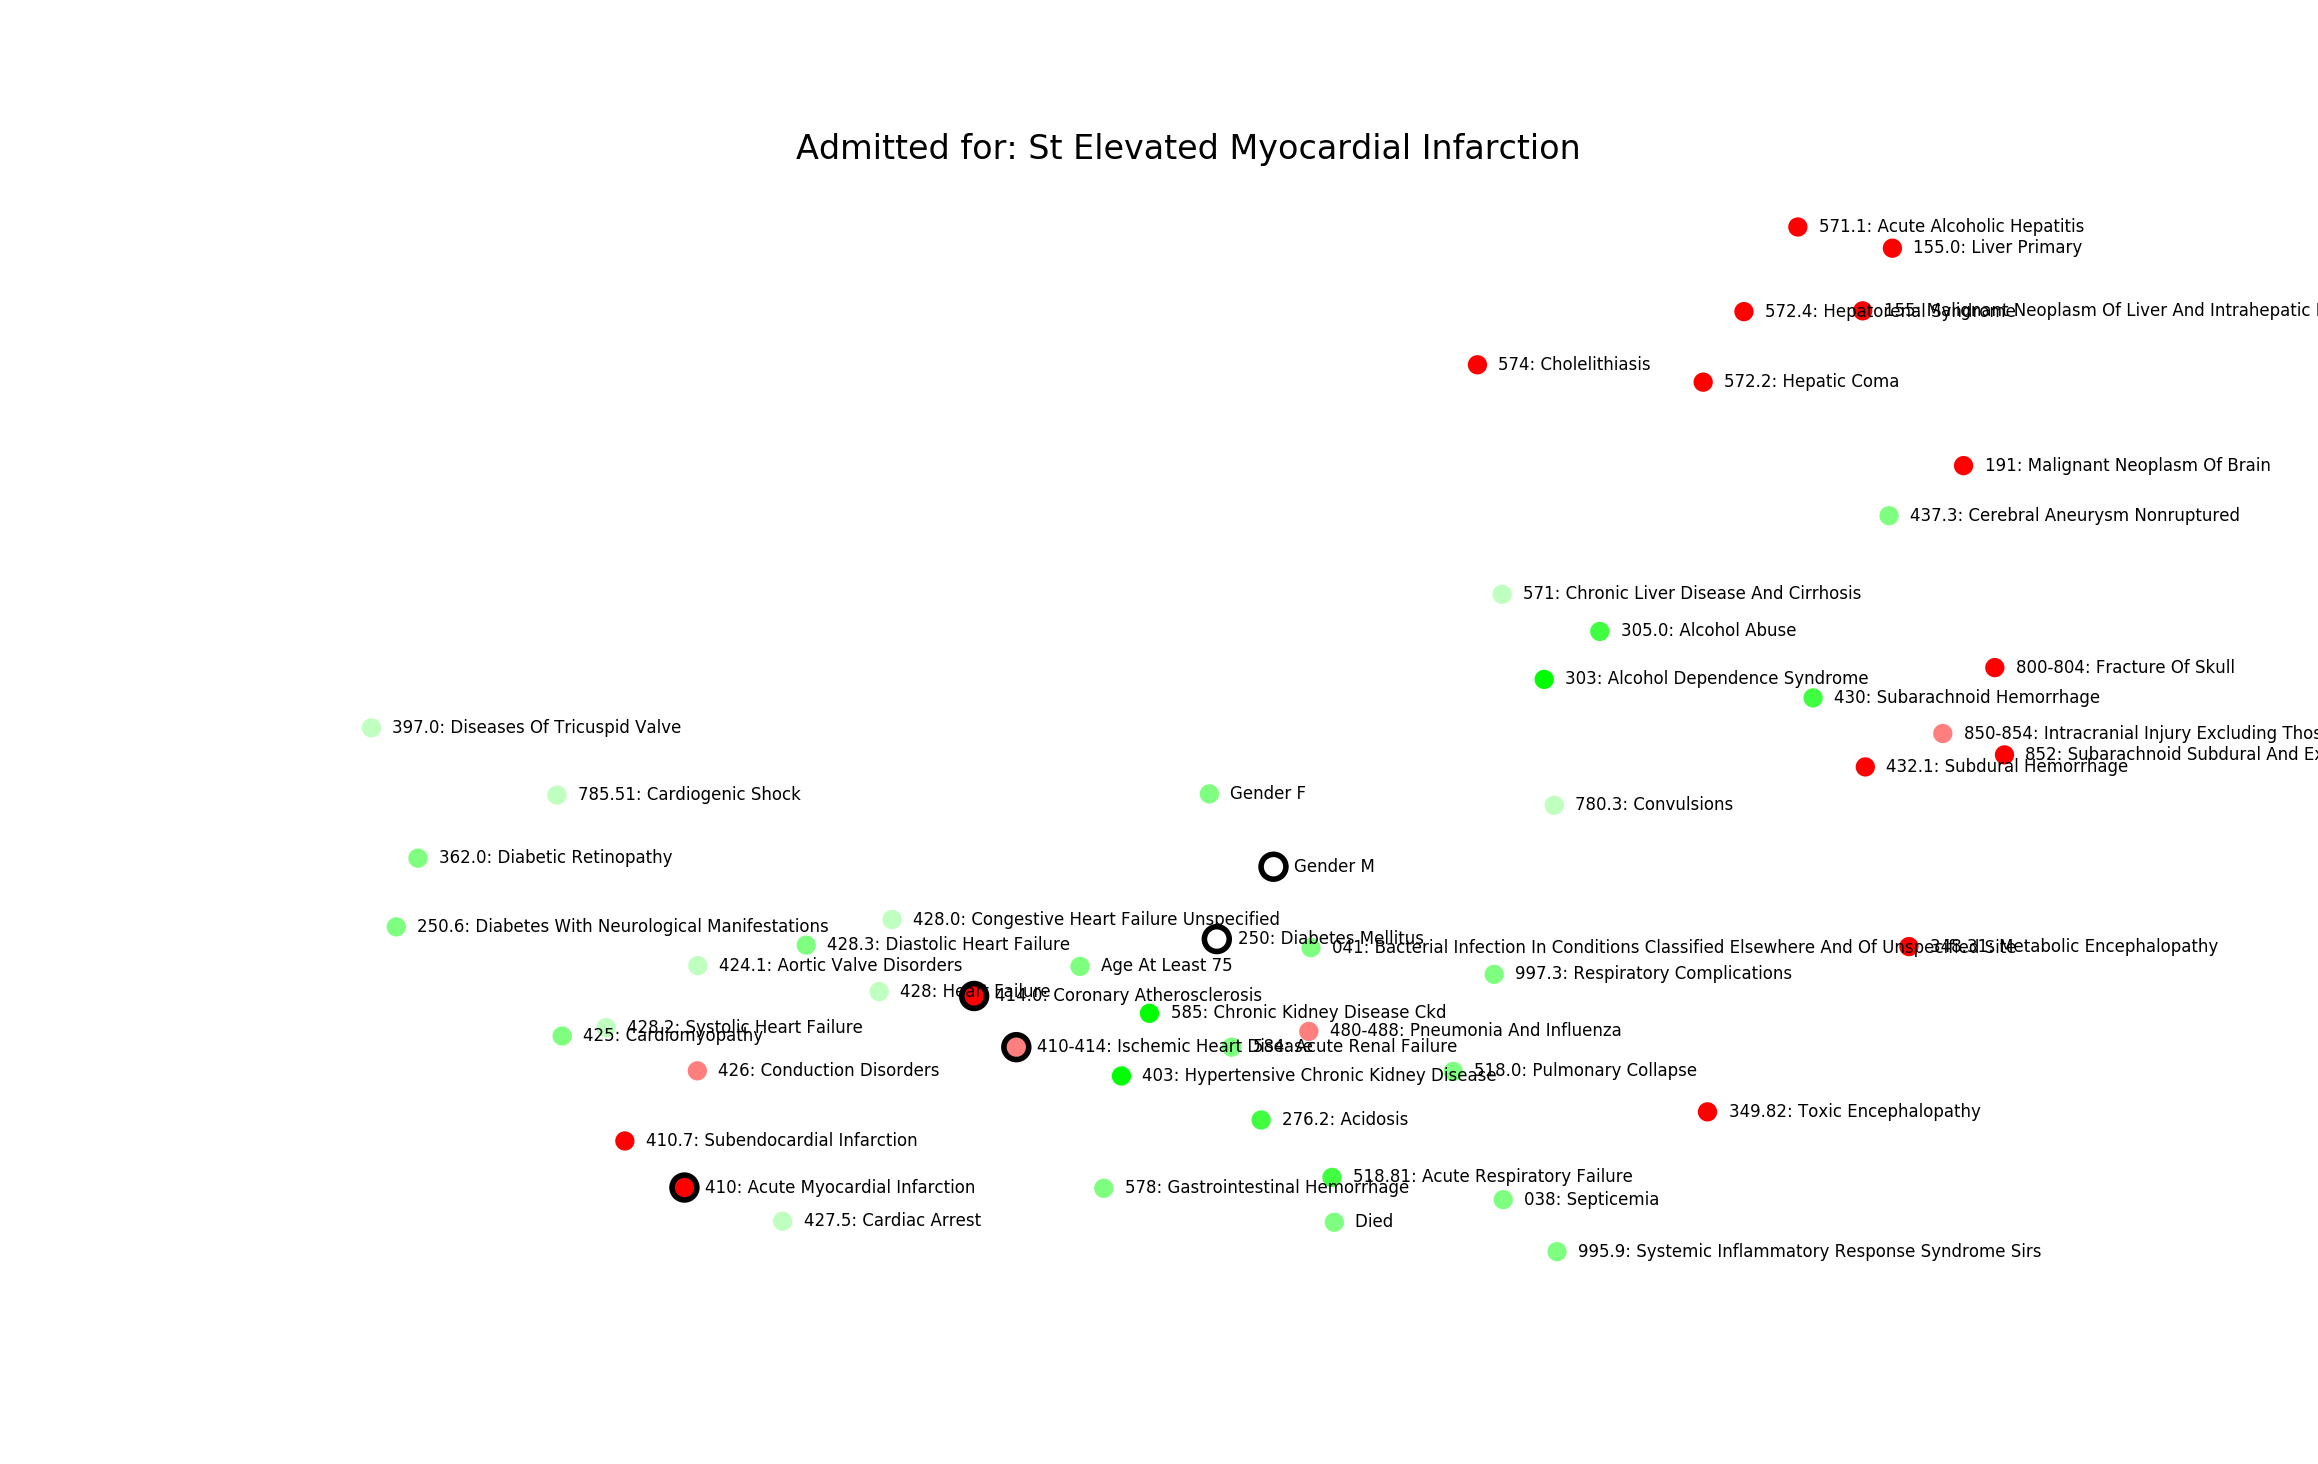
\includegraphics[width=\textwidth]{icu_map_mi}
\caption{Semantic Inference Myocardial Infarction}
\vspace{12px}
Insert caption here
\label{fig:icu_map_mi}
\end{figure}

\begin{figure}
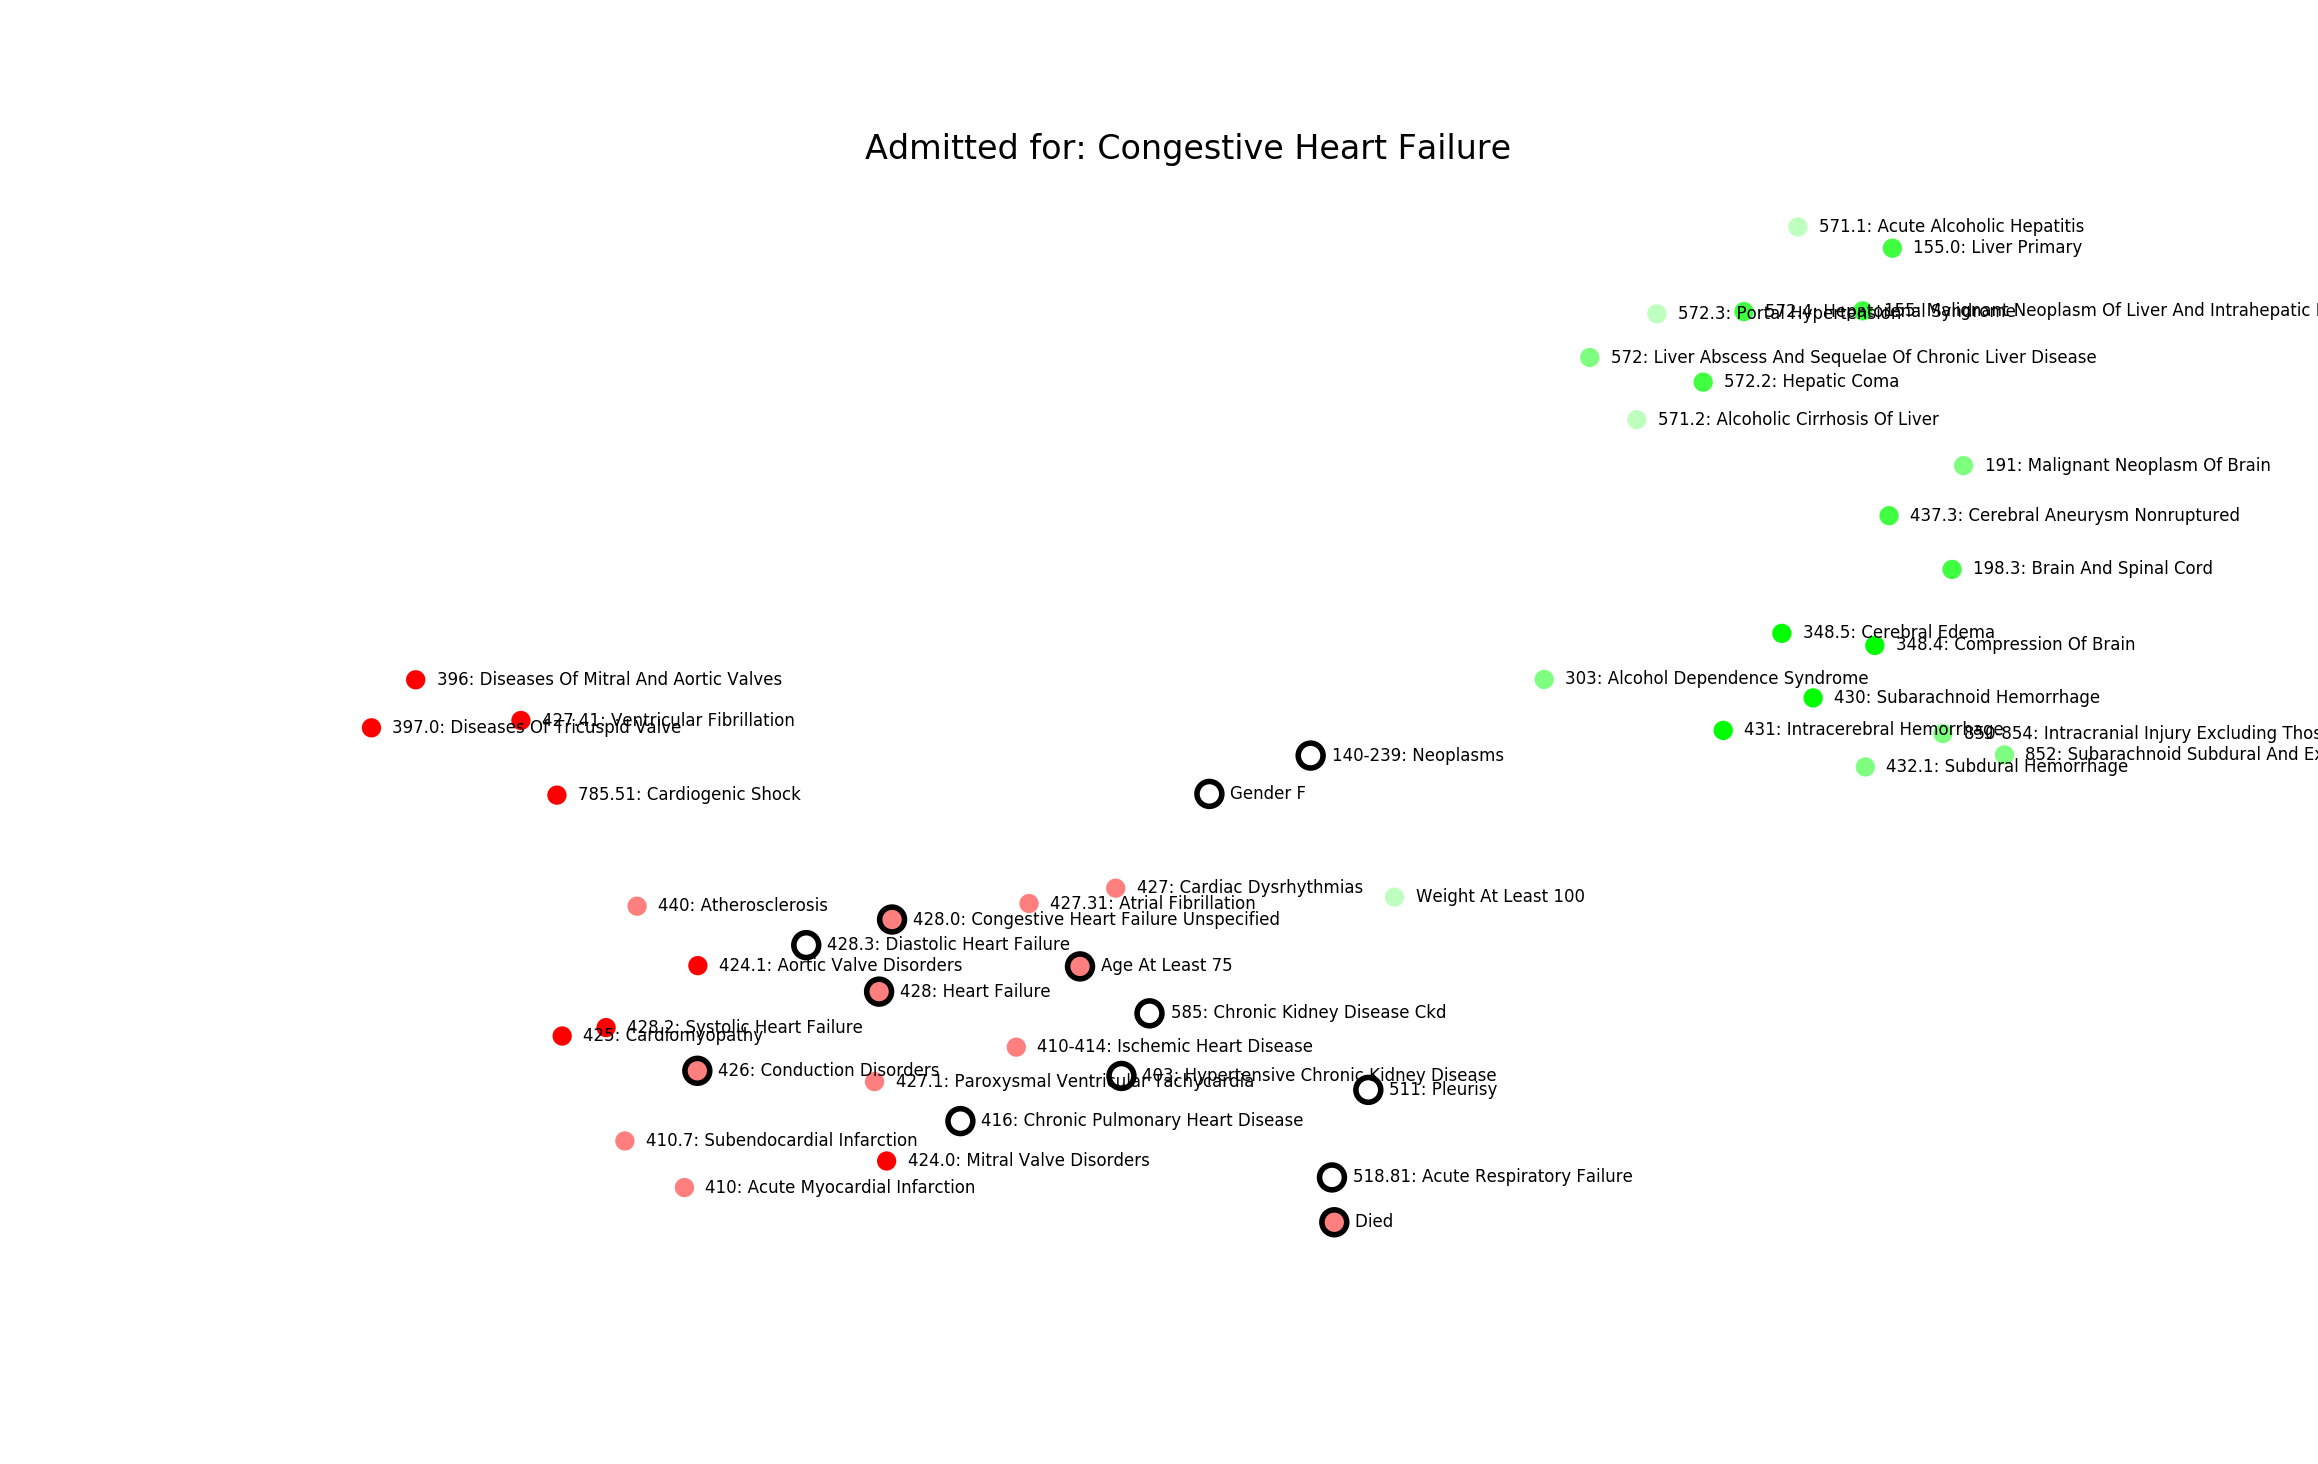
\includegraphics[width=\textwidth]{icu_map_chf}
\caption{Semantic Inference Congestive Heart Failure}
\vspace{12px}
Insert caption here
\label{fig:icu_map_chf}
\end{figure}

\begin{figure}
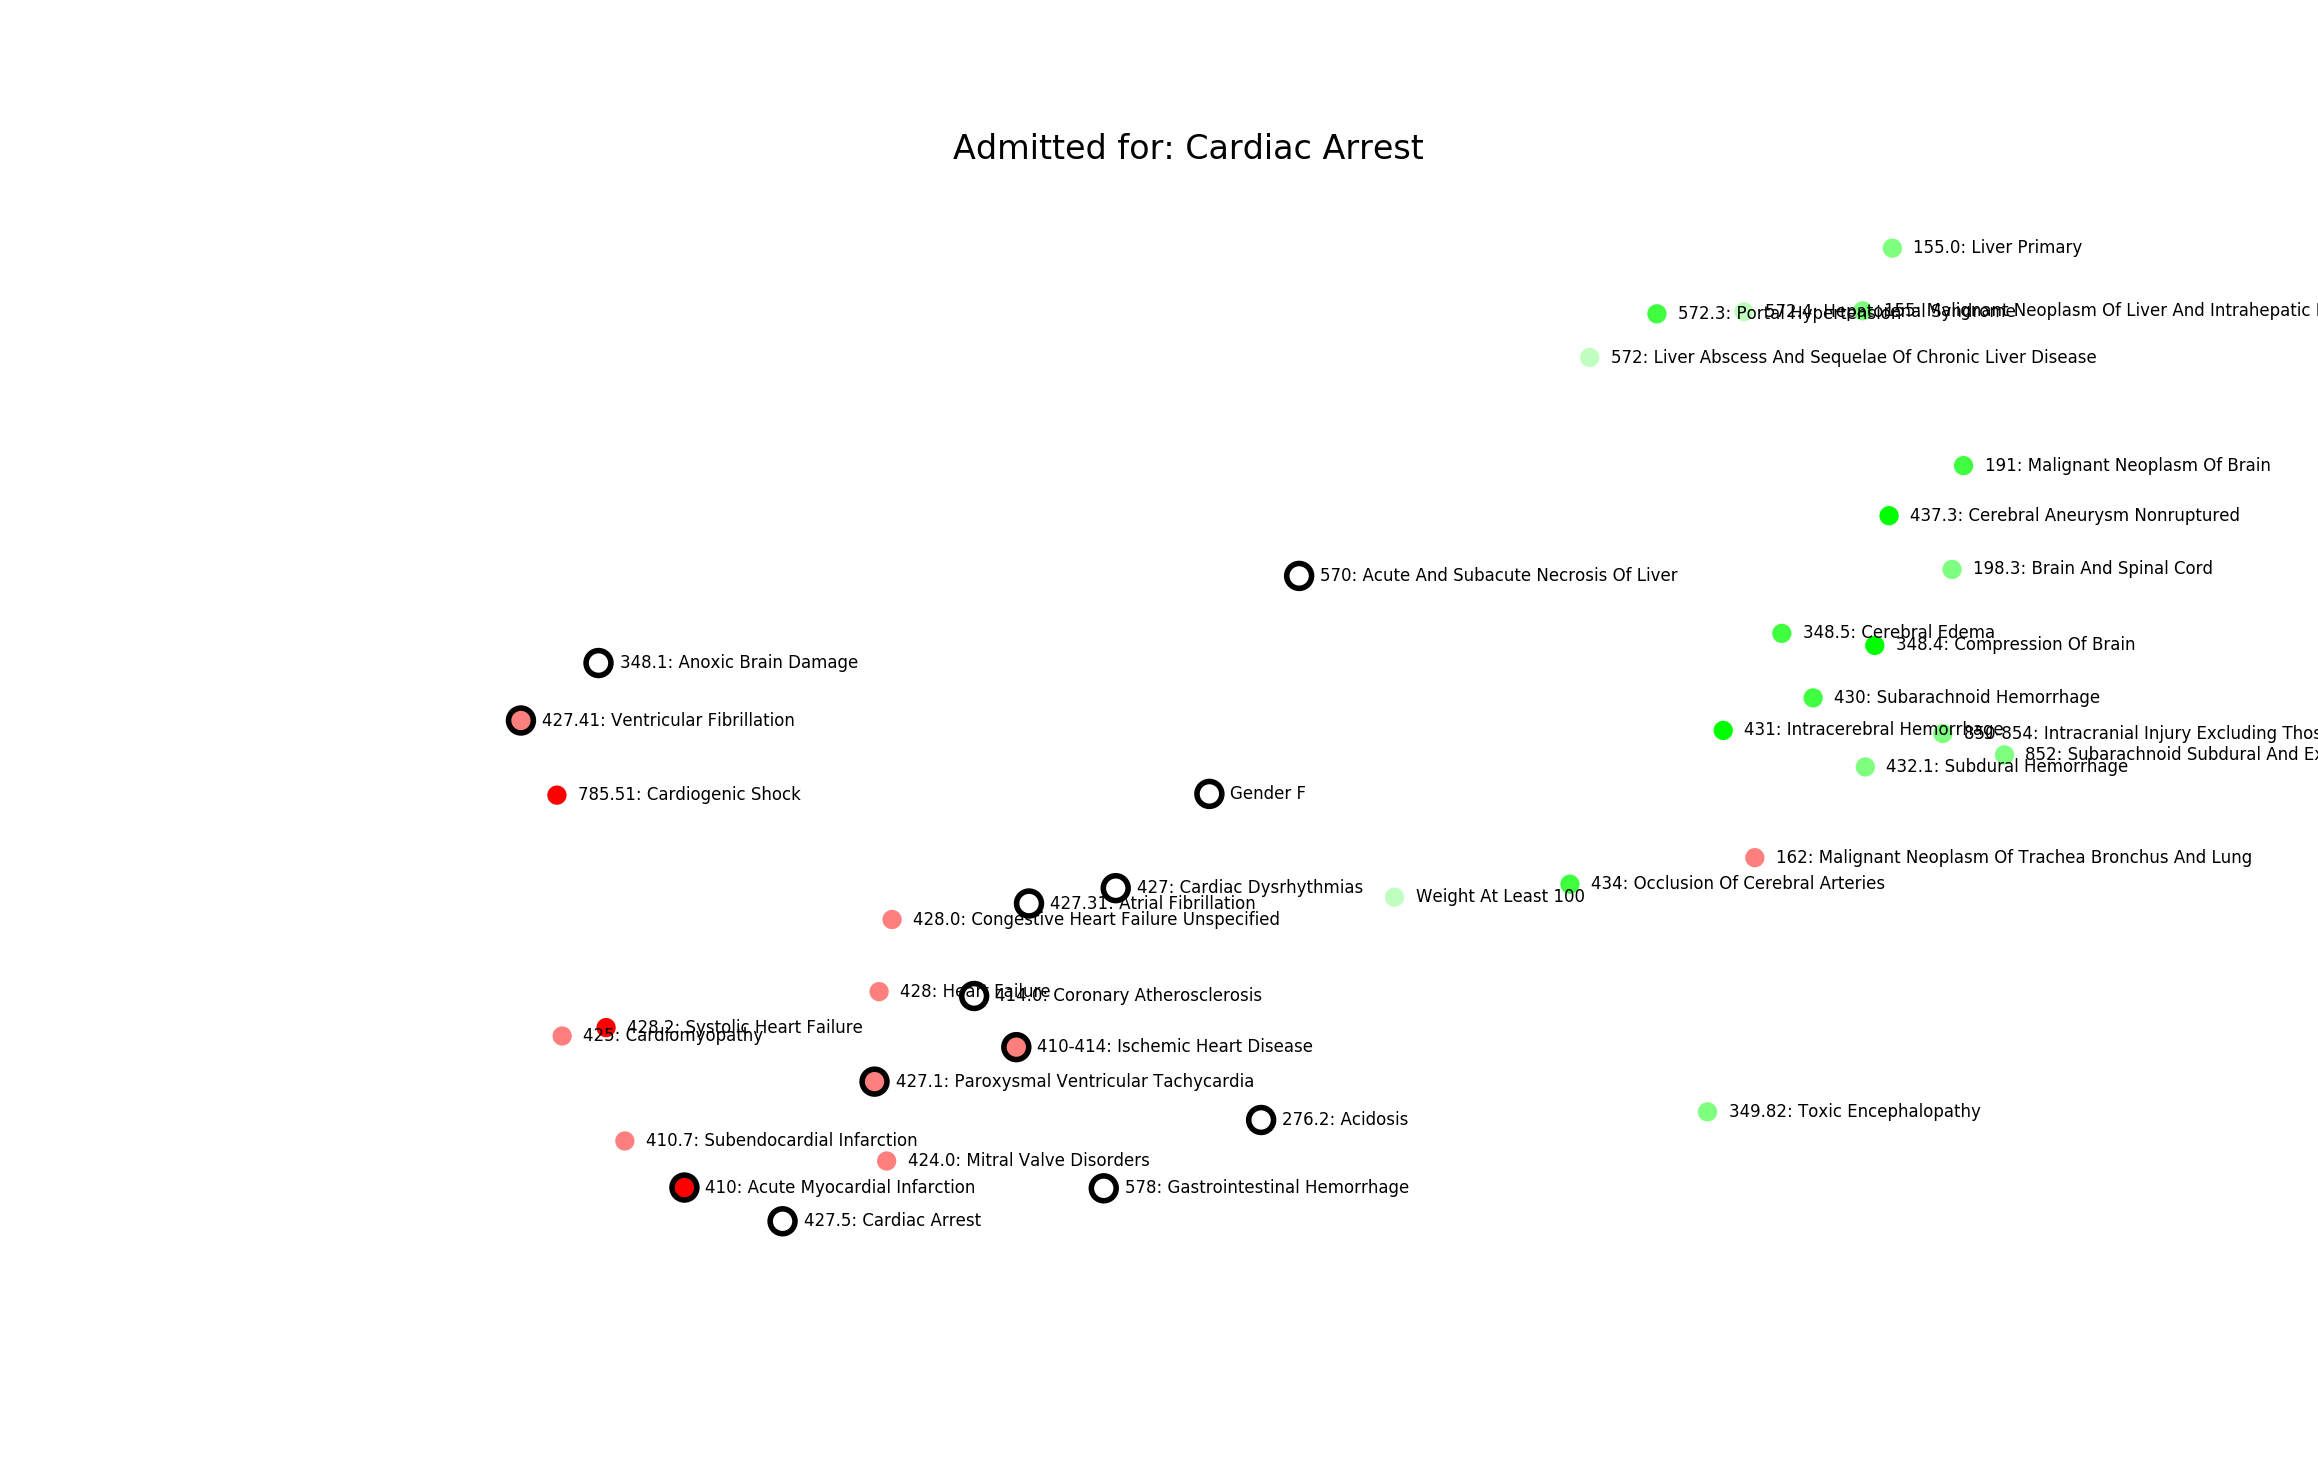
\includegraphics[width=\textwidth]{icu_map_cardarr}
\caption{Semantic Inference Cardiac Arrest}
\vspace{12px}
Insert caption here
\label{fig:icu_map_cardarr}
\end{figure}

\begin{figure}
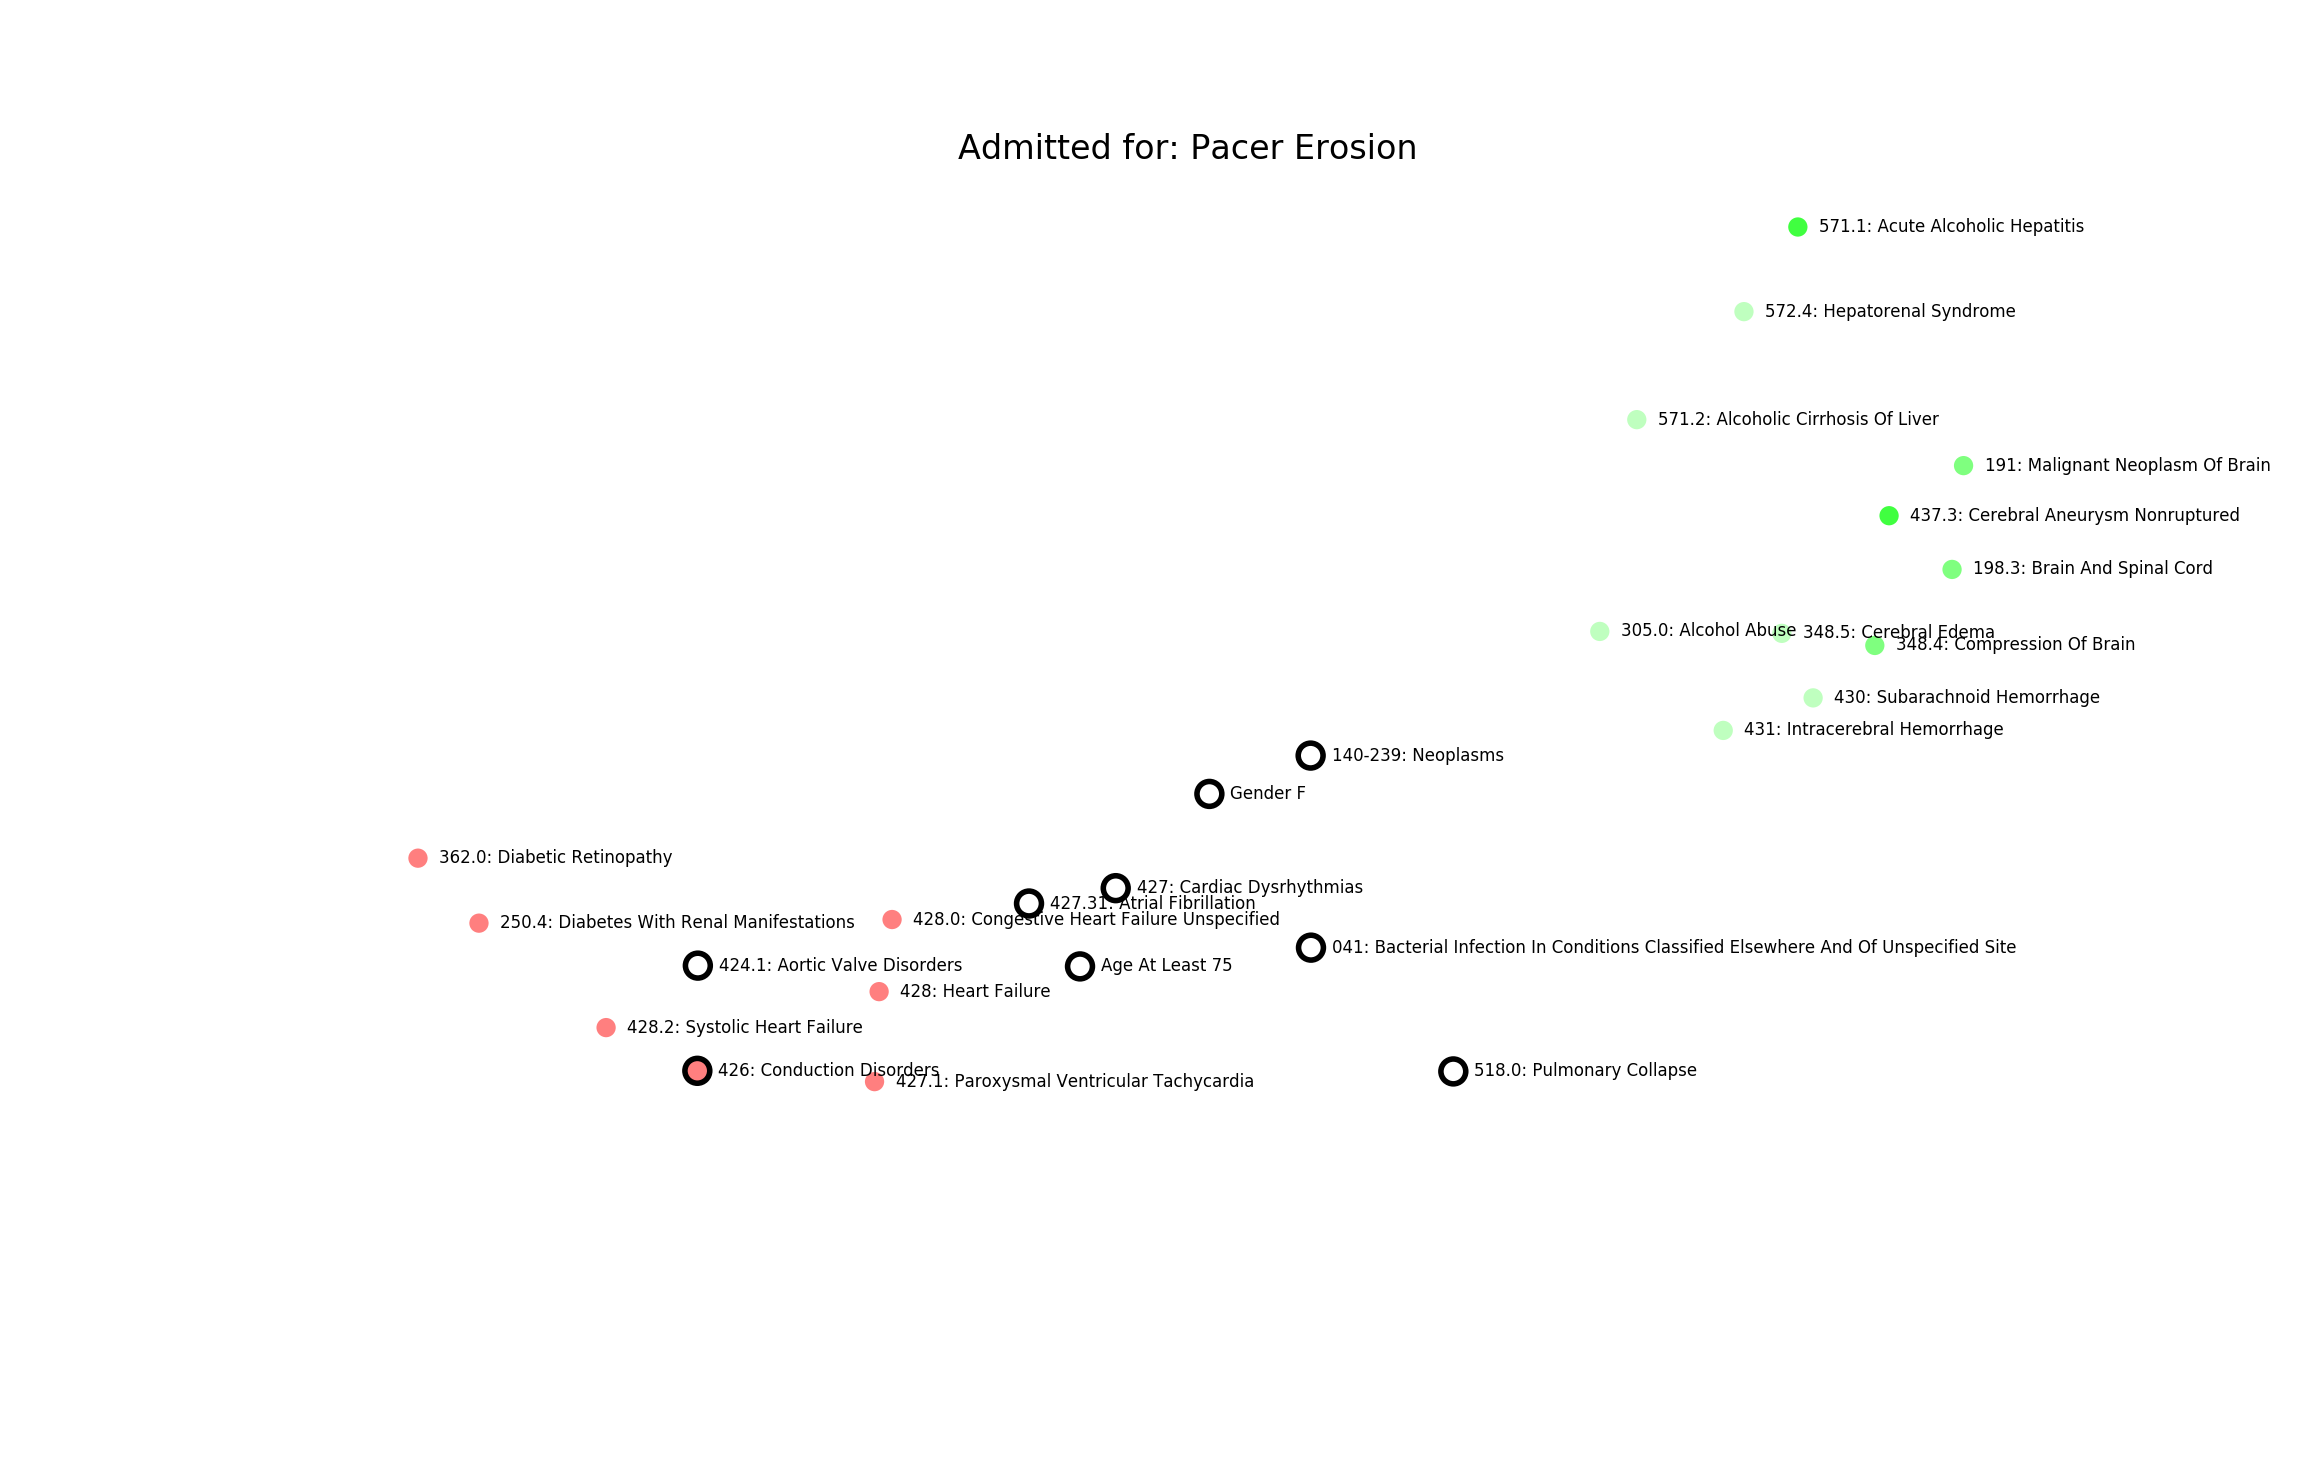
\includegraphics[width=\textwidth]{icu_map_pacer}
\caption{Semantic Inference Pacer Erosion}
\vspace{12px}
Insert caption here
\label{fig:icu_map_pacer}
\end{figure}

\begin{figure}
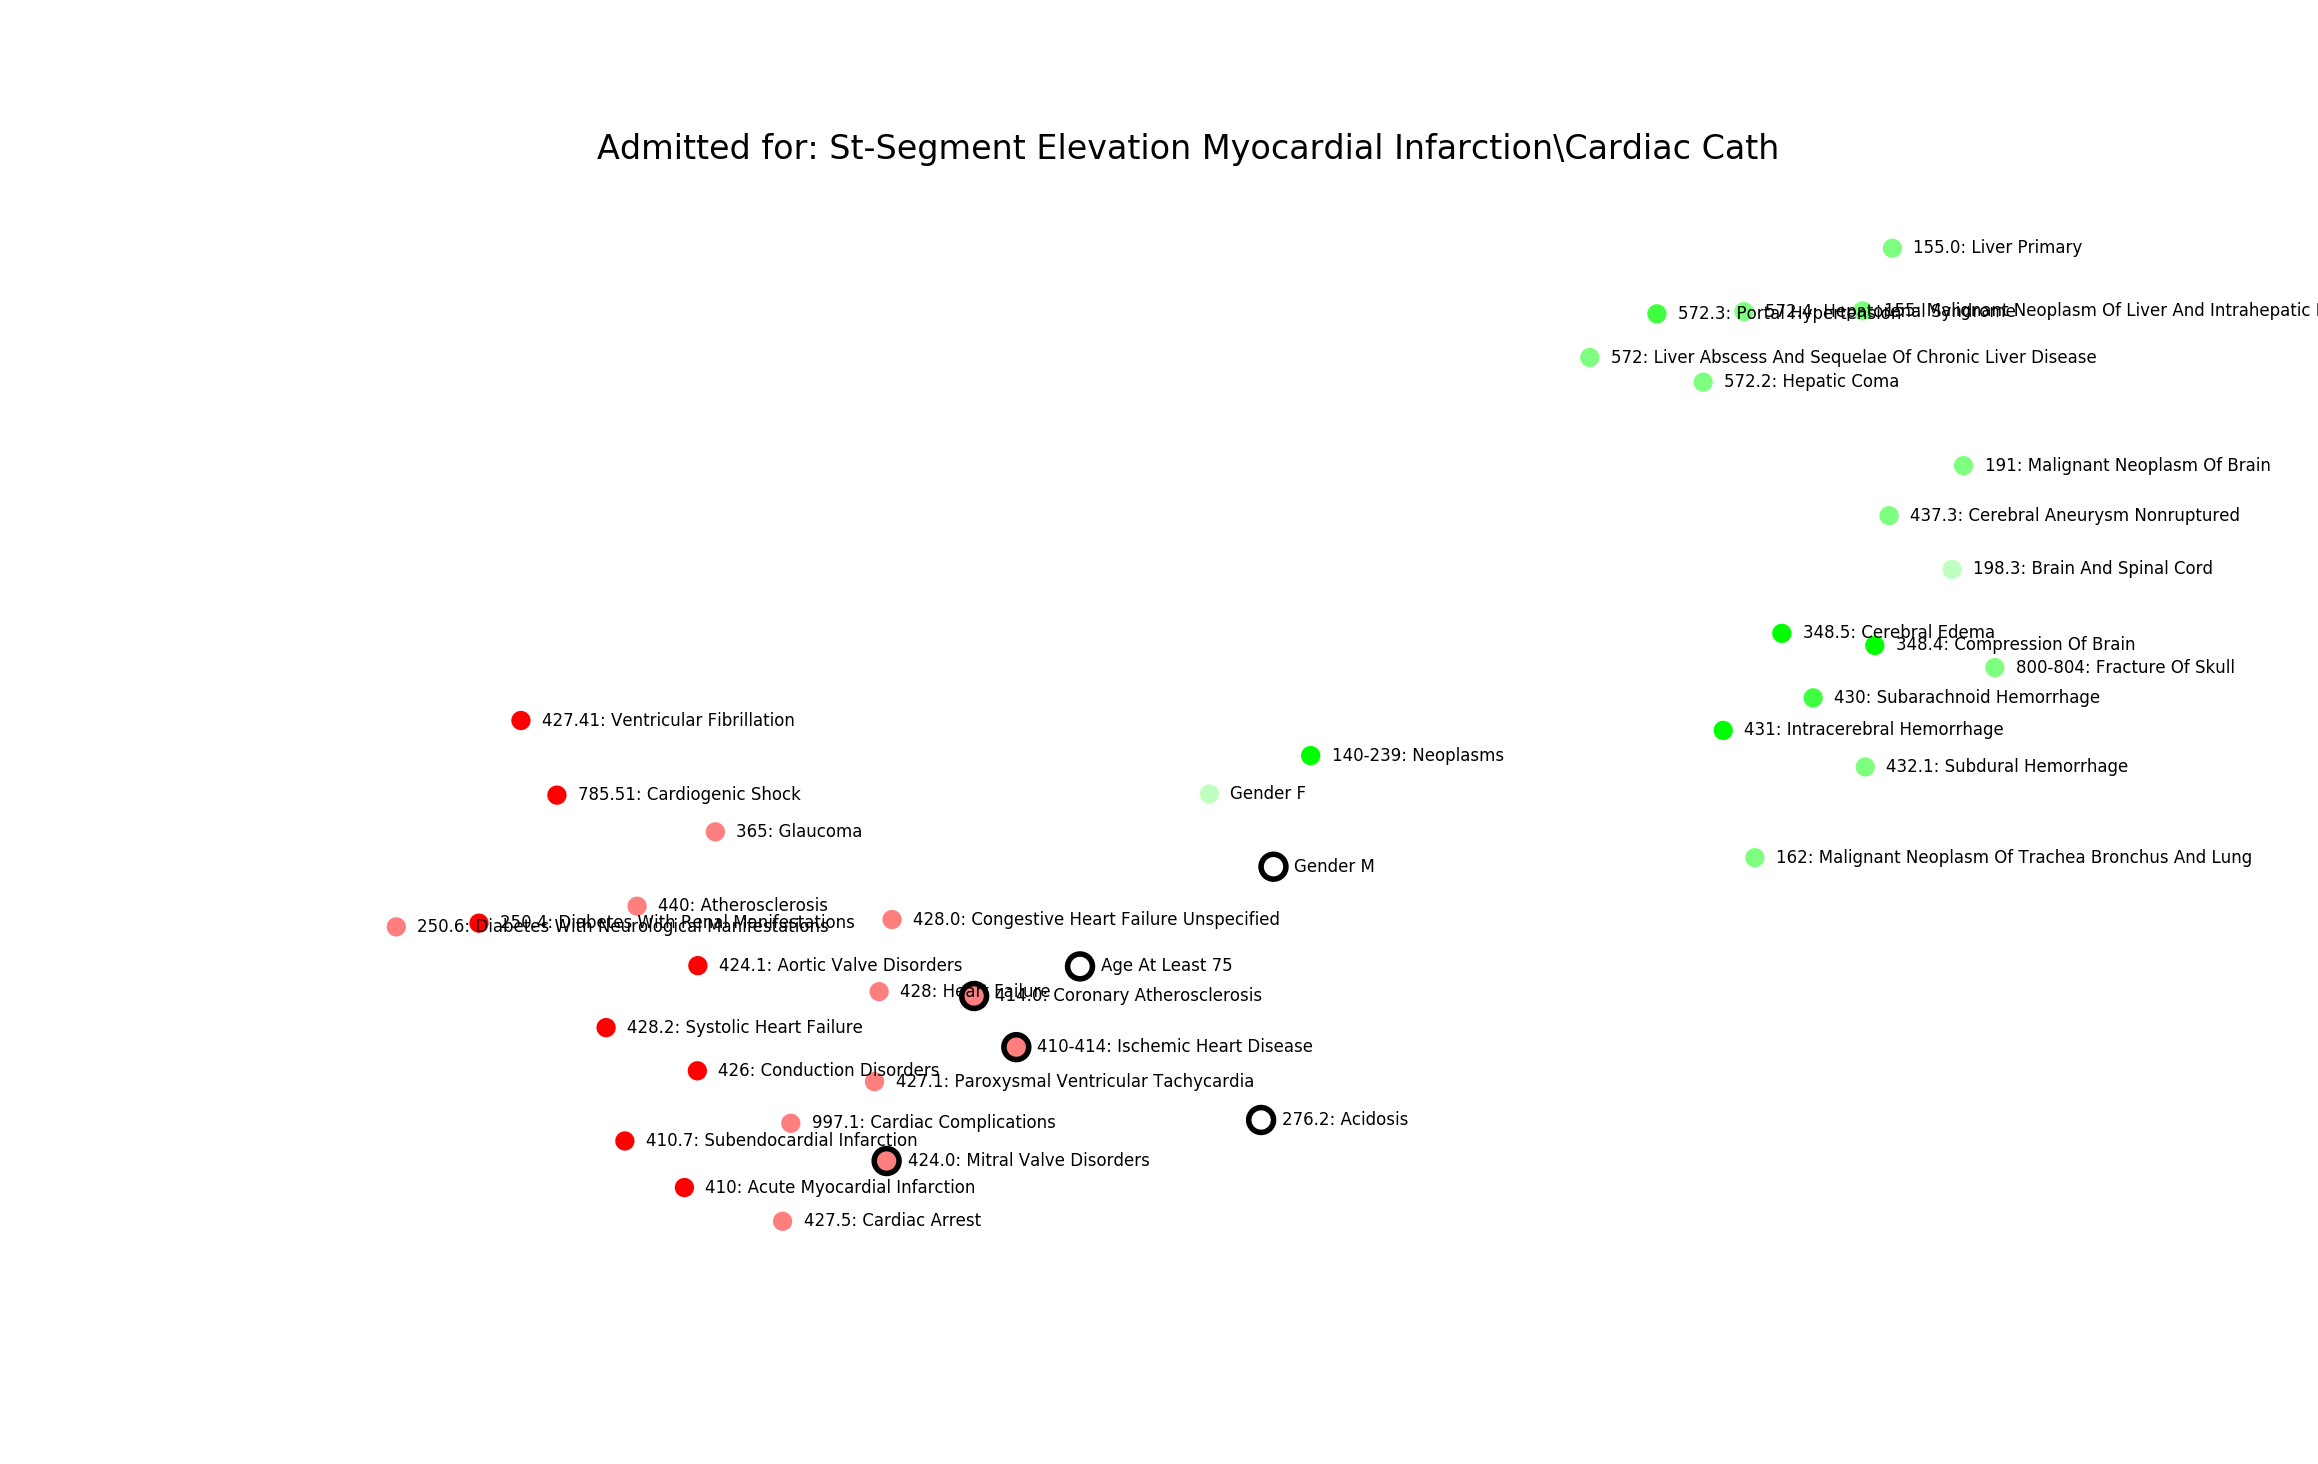
\includegraphics[width=\textwidth]{icu_map_stseg}
\caption{Semantic Inference ST Elevation}
\vspace{12px}
Insert caption here
\label{fig:icu_map_stseg}
\end{figure}

\begin{figure}
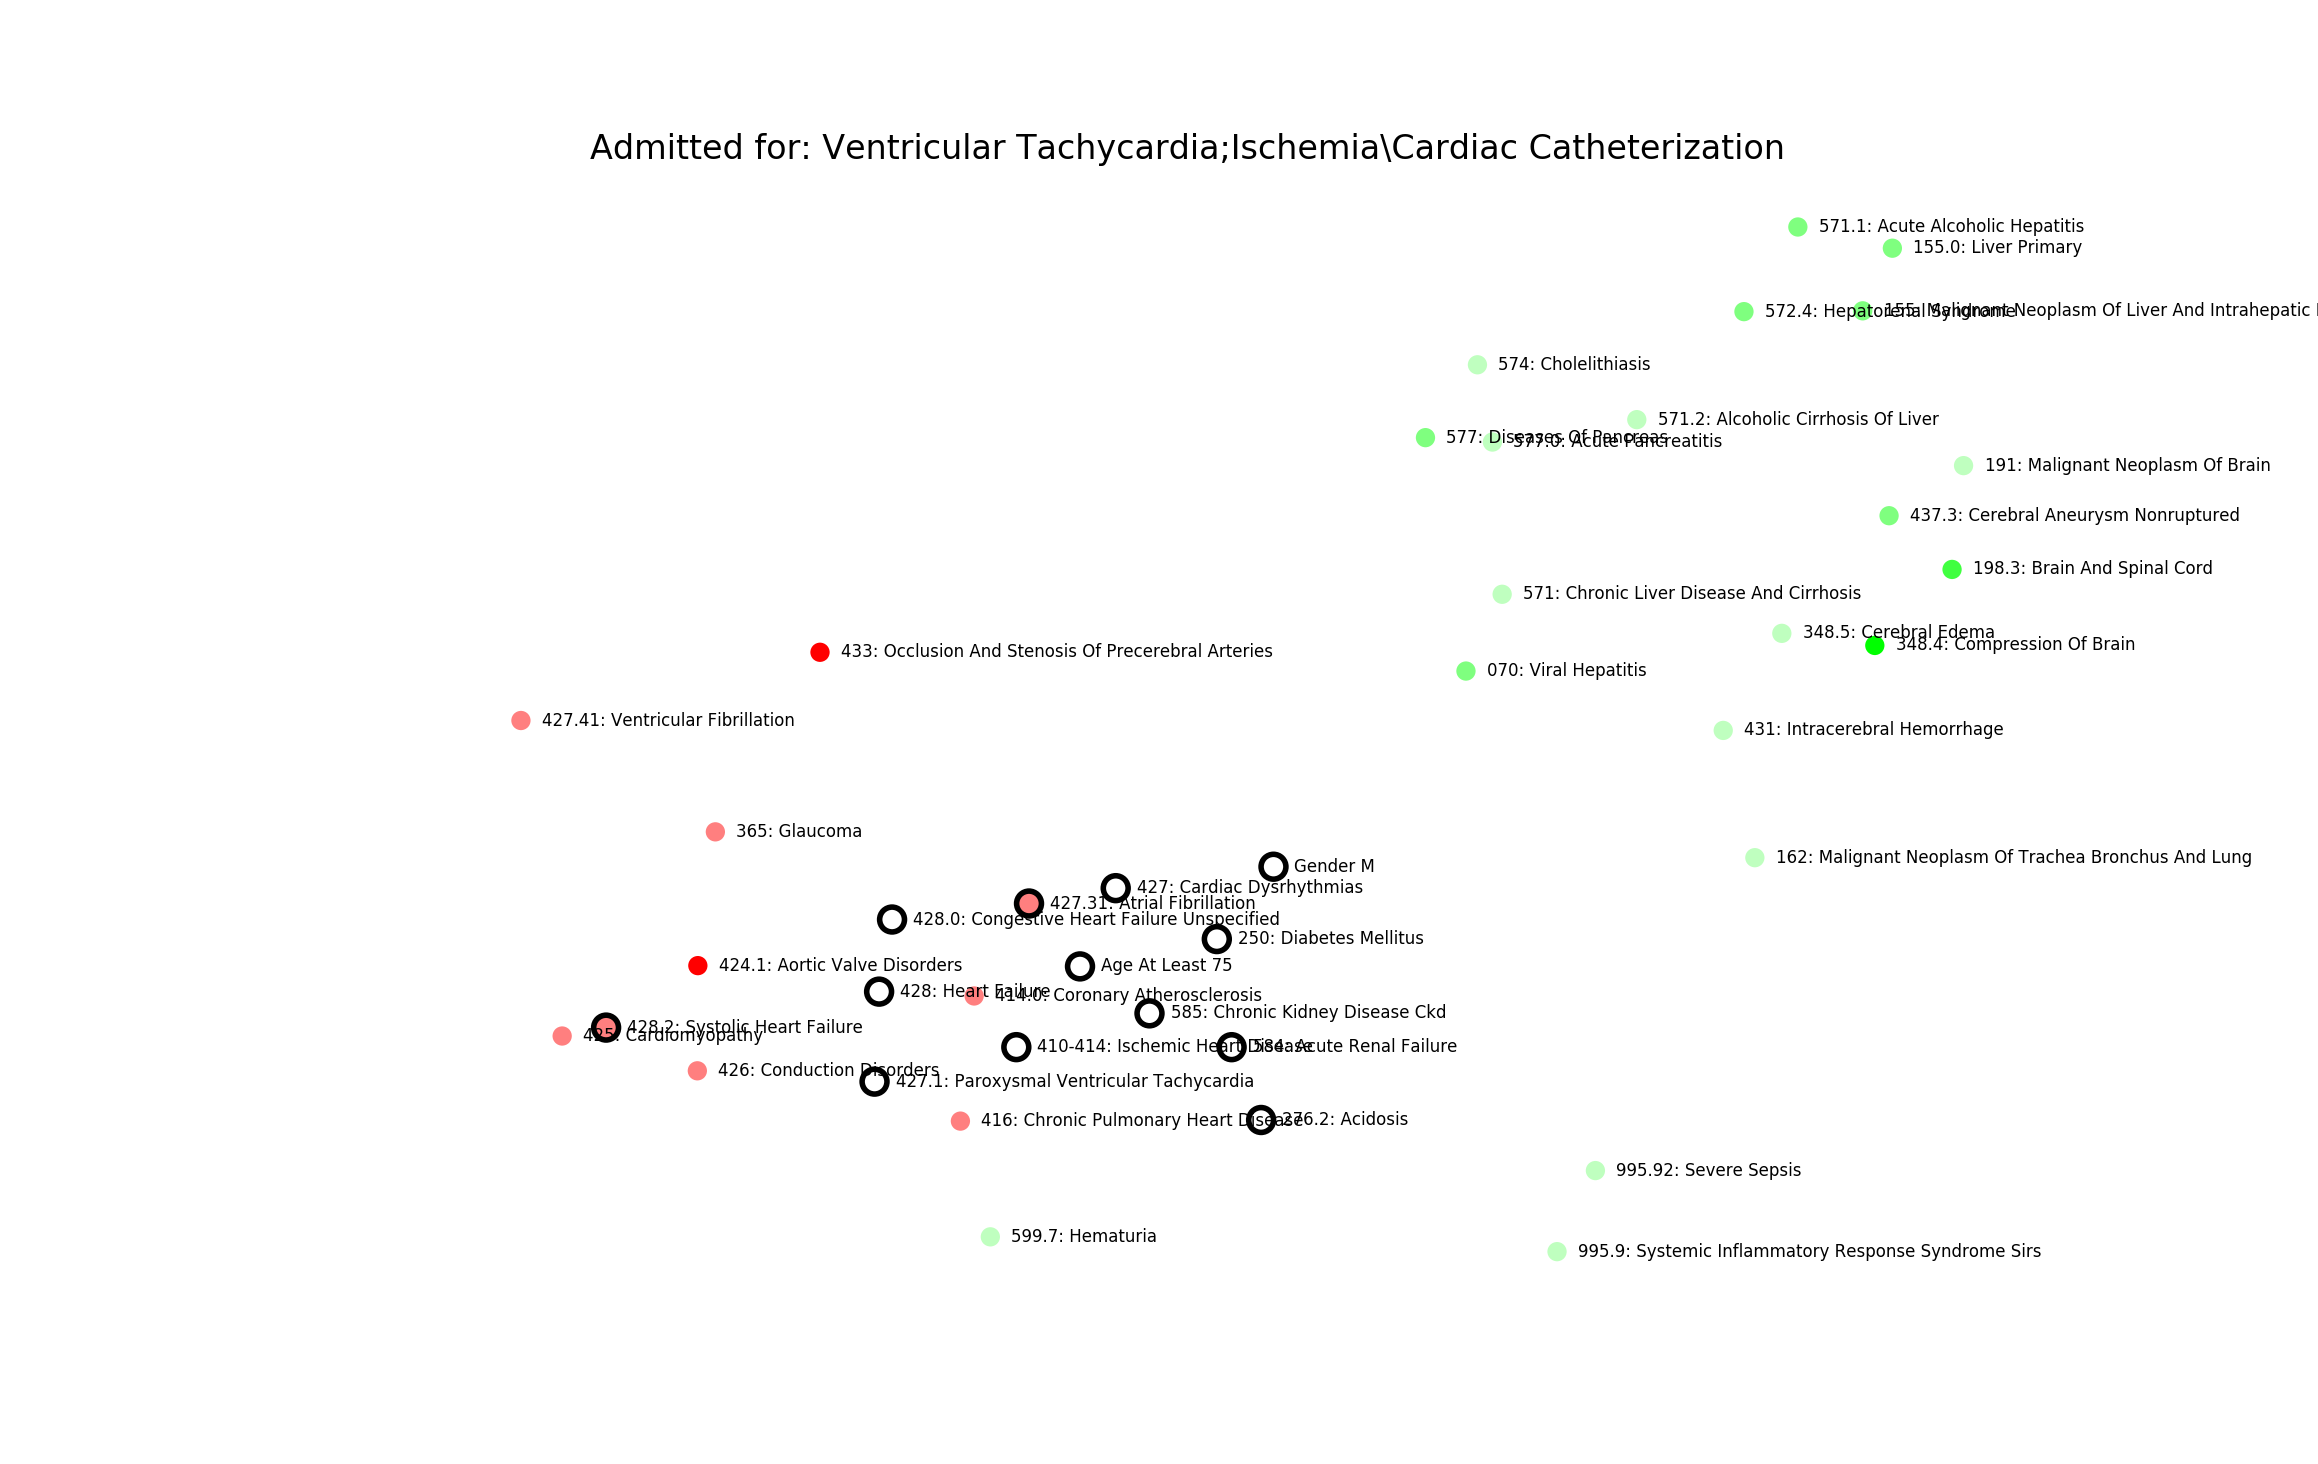
\includegraphics[width=\textwidth]{icu_map_ventach}
\caption{Semantic Inference Ventricular Tachycardia}
\vspace{12px}
Insert caption here
\label{fig:icu_map_ventach}
\end{figure}

\begin{figure}
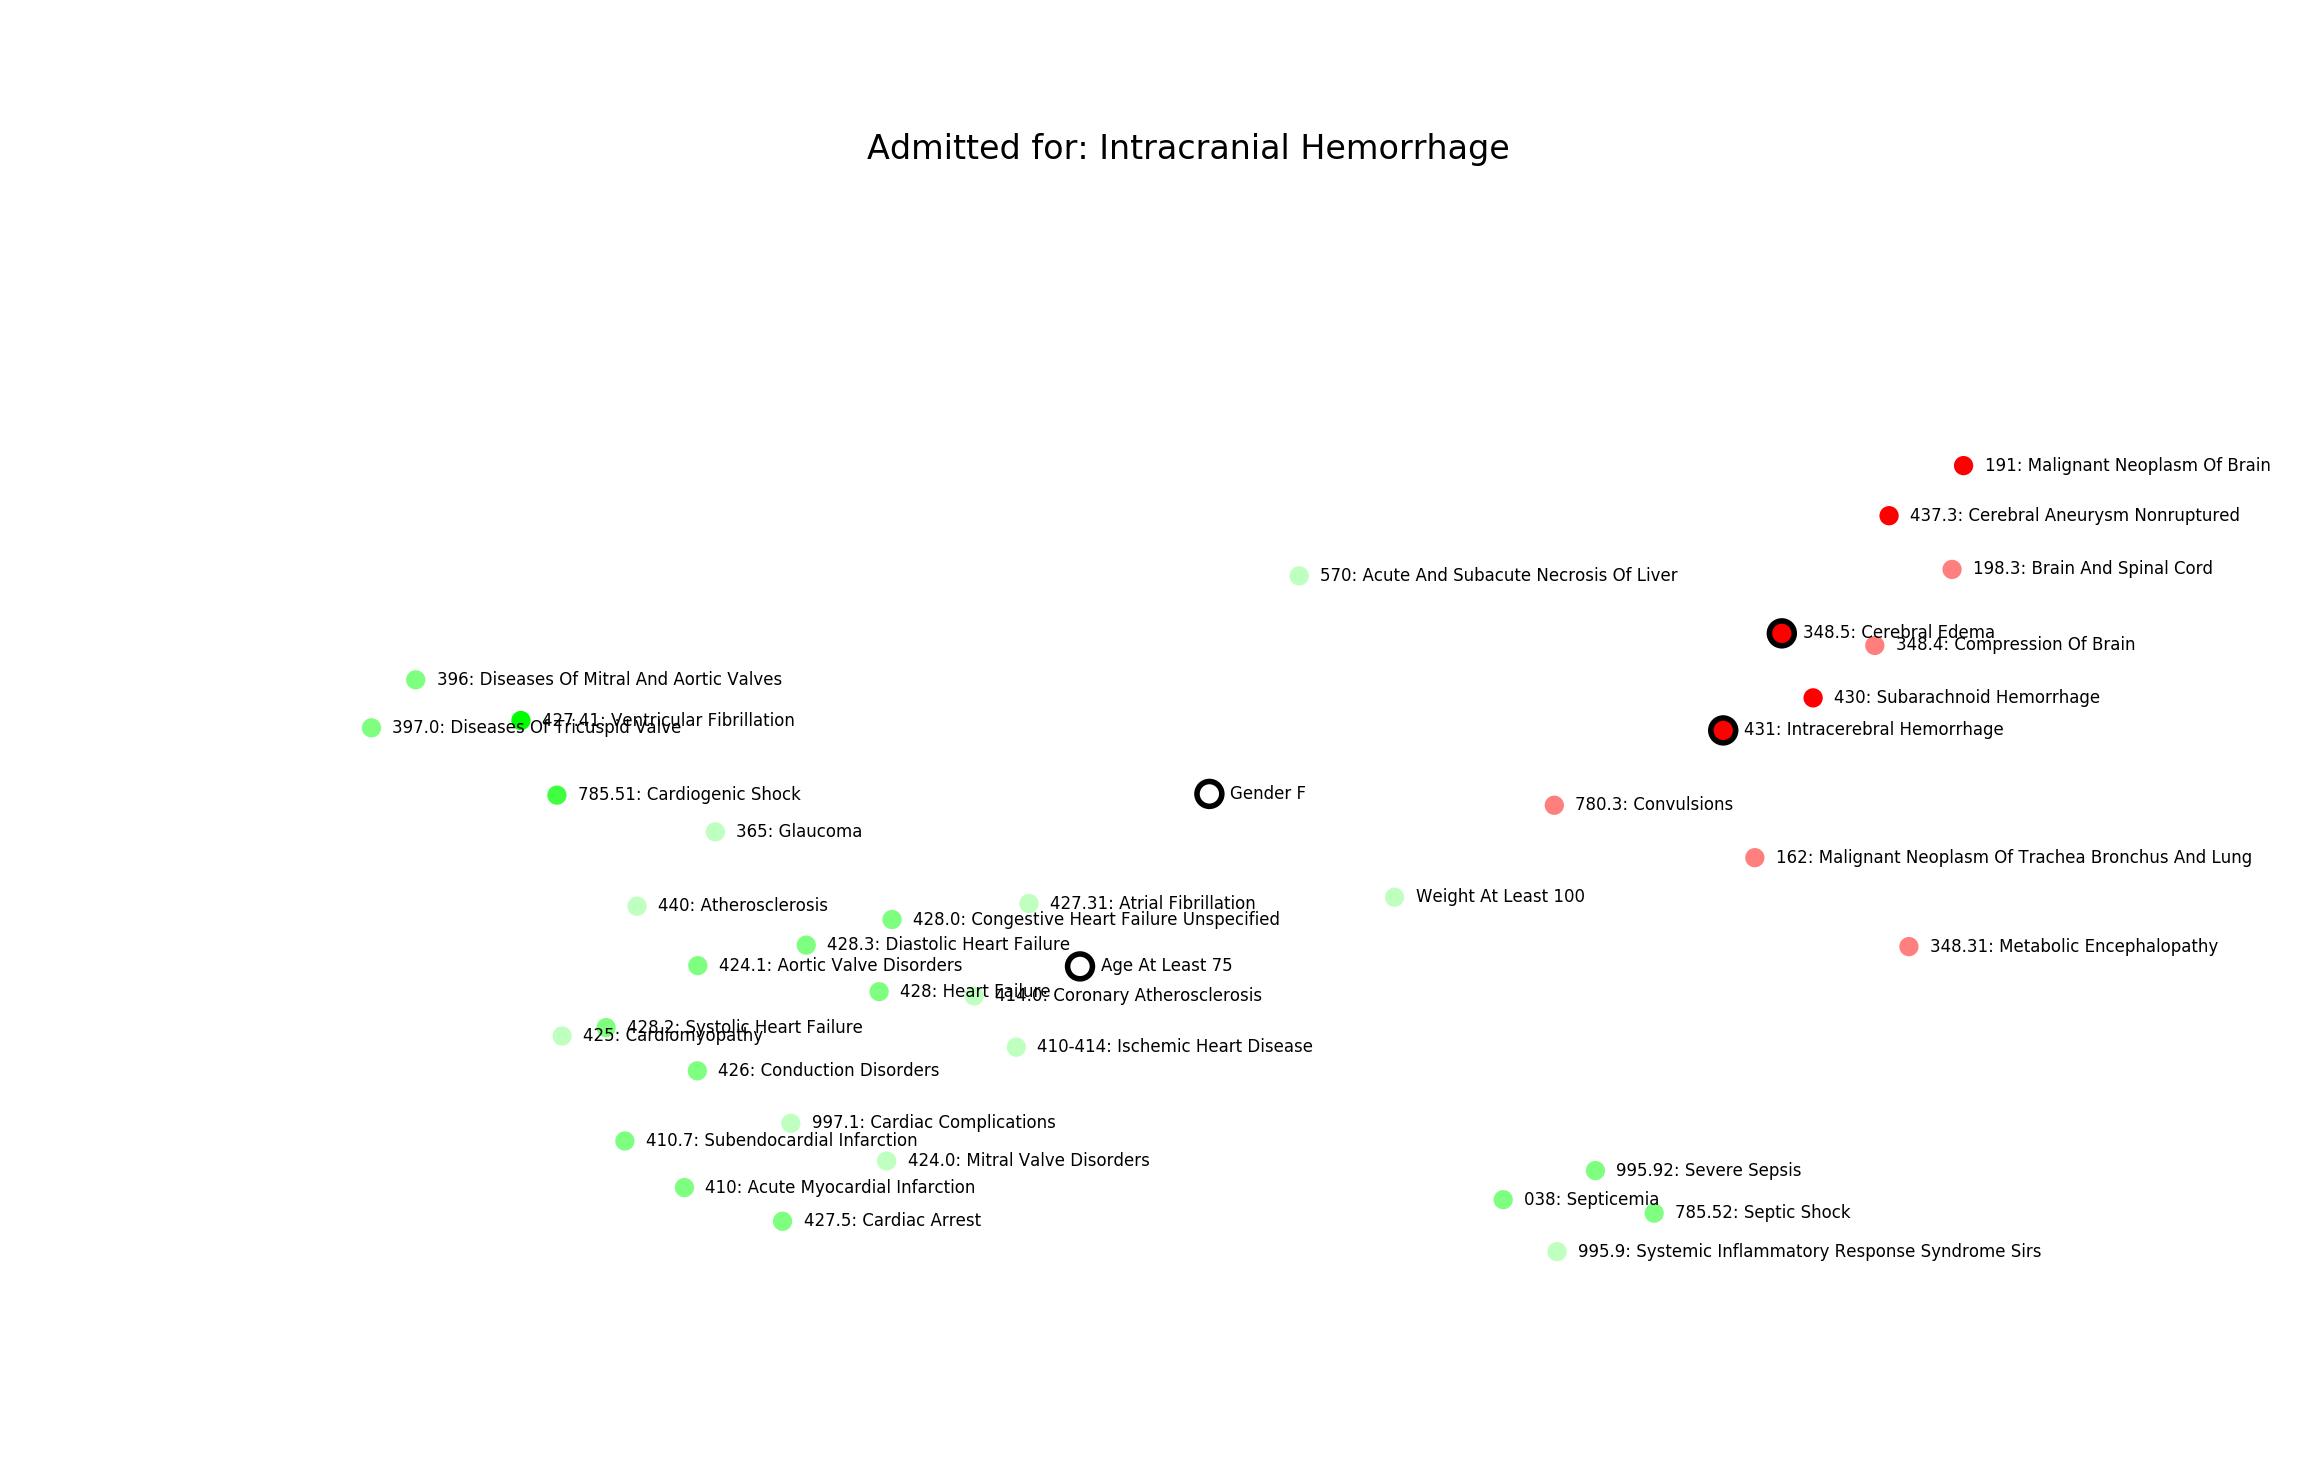
\includegraphics[width=\textwidth]{icu_map_brain}
\caption{Semantic Inference Intracranial Hemorrhage}
\vspace{12px}
Insert caption here
\label{fig:icu_map_brain}
\end{figure}

\begin{figure}
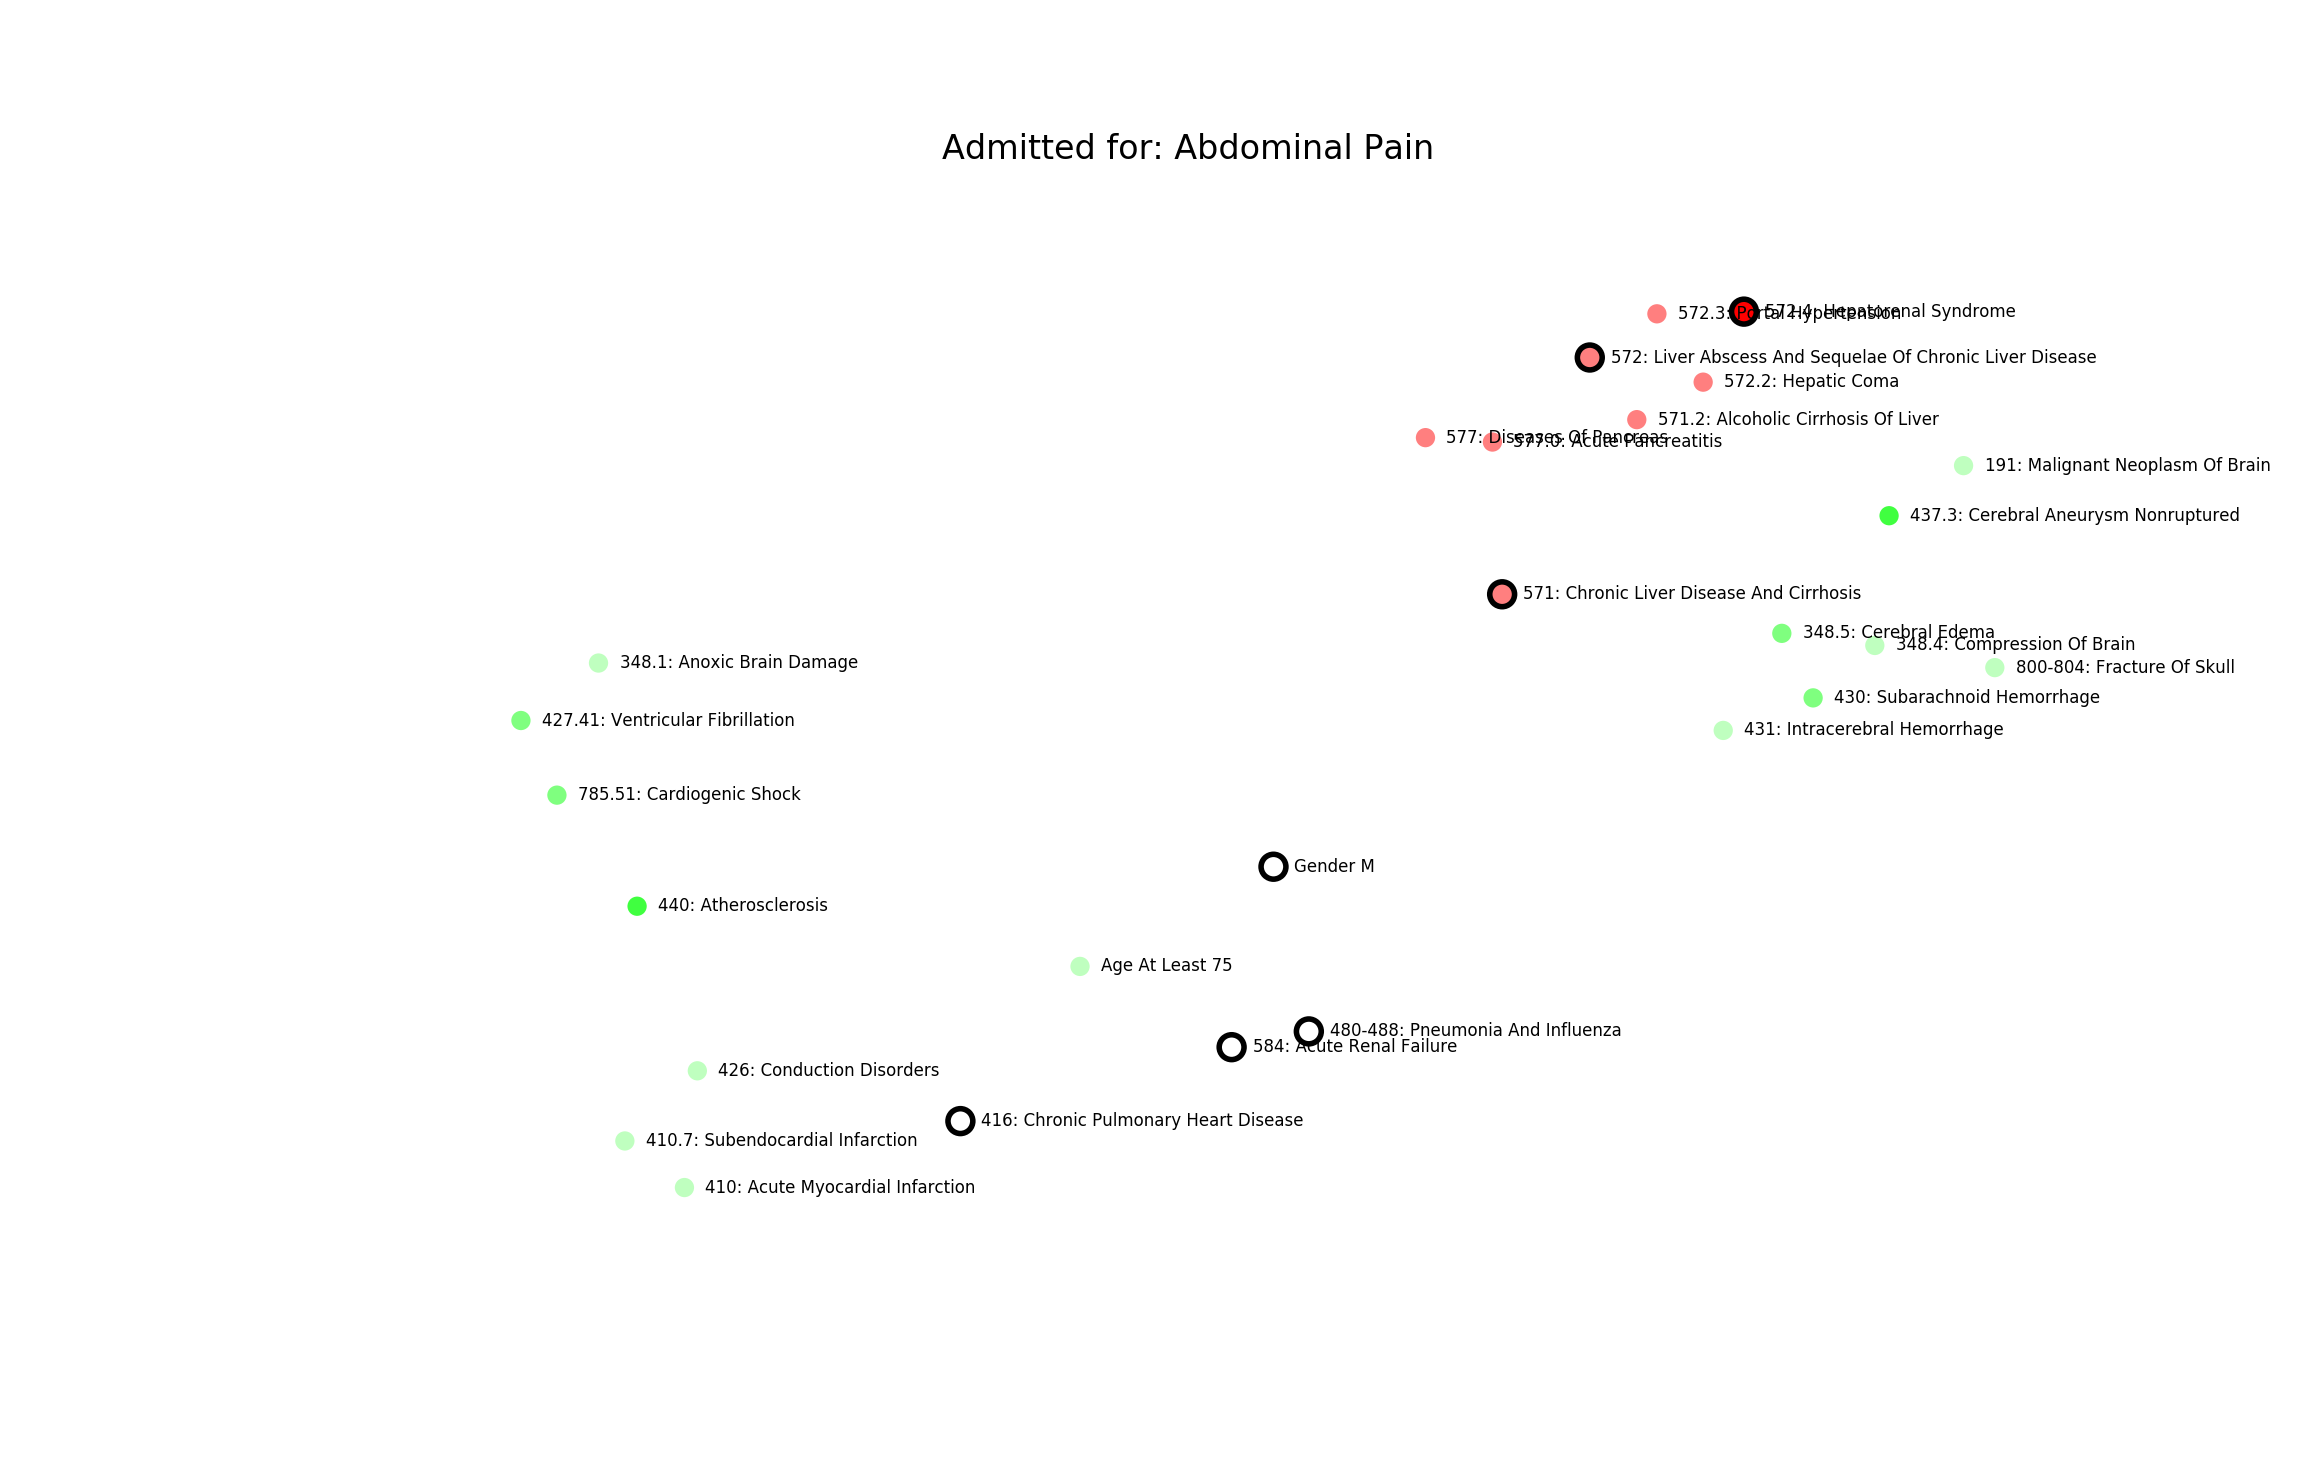
\includegraphics[width=\textwidth]{icu_map_liver}
\caption{Semantic Inference Abdominal Pain}
\vspace{12px}
Insert caption here
\label{fig:icu_map_liver}
\end{figure}

\section{Introduction}
Admission to the intensive care unit (ICU) in hospitals is associated with risk of acute mortality given critical illness for those patients, which can include shock and end organ damage. During this period, patients are closely monitored in the intensive care setting with both invasive and noninvasive sensor data and frequent lab monitoring in order to effectively determine and prevent complications of critical illness.  Physicians often use risk scores designed to identify and predict patients’ risk of conditions such as shock: general physiologic scoring like shock index, or more specifically septic shock (qSOFA score) or cardiogenic shock (completing Fick’s formula for cardiac index, cardiac output, and stroke volume).

Wearable devices are becoming more and more common.  Over 100 million people wear an Apple Watch.  This device is capable of measuring both a photoplethysmogram (PPG) and an electrocardiogram (ECG).  While data for this device is not yet openly available in large quantities, there are large amounts of data available for patients in critical care.  These datasets include waveforms measured in the ICU, which include the waveforms measured by an Apple Watch.  This distribution of patients in an ICU vs the average Apple Watch user are admittedly different.  As demonstrated in chapter 1 though, a lot can be gained from first training on a large related dataset (e.g. cats and dogs) and then fine-tuning on the dataset of interest (e.g. skin lesions).  For this situation, we use the MIMIC ICU dataset in a similar manner as ImageNet.  A further study could fine-tune this model on data collected from Apple Watch users.

\section{Dataset}
The dataset used was collected by MIT.  It is essentially a data dump of data collected from the hospital, far from the pristine labeled ImageNet dataset.  Much care was needed to transform it into a form that a neural net could be trained with.  The dataset includes over 60 thousand ICU patients.  For each hospital admission a variable number of waveforms are recorded.  Additionally each patient was diagnosed with a variable number of conditions as evidenced by the ICD codes on their chart.

\subsection{ICD Codes}
TODO

\subsection{Inputs}
TODO

\section{Model Architecture}
TODO

\section{Effective Sensitivity}
Expensive vs Ubiquitous

\subsection{Definition}
TODO

\subsection{Results}
TODO

\section{Relative Risk}
TODO

\subsection{Definition}
TODO

\subsection{Results}
TODO

\section{Semantic Space Inference}
TODO

\subsection{Definition}
TODO

\subsection{Results}
TODO